\documentclass[11pt, oneside]{article}  
\usepackage[margin=0.5in]{geometry} % Margins
\usepackage[ampersand]{easylist} % Bullets for lists
\usepackage[bottom]{footmisc}  % Glue footnotes to bottom
\usepackage{graphicx}
\graphicspath{ {imgs/} }

\title{Operating Systems Principles\\UCLA-CS111-W18}
\author{Quentin Truong\\Taught by Professor Reiher}
\date{Winter 2018}


\begin{document}
\maketitle
\tableofcontents
\pagenumbering{arabic}
\clearpage


%========================================================
\section{L3: Arpaci-Dusseau Chapter 5: Interlude: Process API}
\subsection{The fork() System Call}
	\begin{easylist}  
	\ListProperties(Hide=100, Hang=true, Progressive=4ex, Style*=--\ , Style2*=$\bullet\ $)
        & Crux: How to create and control processes
		& fork()
        && Creates new process; returns child's PID to parent; returns 0 to child;
        && Each has own PC, registers, address space
        & Nondeterministic Behavior
        && Scheduler will decide which process to run
        && May lead to problems in multi-threaded programs
	\end{easylist}

\subsection{The wait() System Call}
    \begin{easylist}  
    \ListProperties(Hide=100, Hang=true, Progressive=4ex, Style*=--\ , Style2*=$\bullet\ $)
        & wait()
        && Parent calls wait() to wait for child to finish execution
    \end{easylist}

\subsection{The exec() System Call}
    \begin{easylist}  
    \ListProperties(Hide=100, Hang=true, Progressive=4ex, Style*=--\ , Style2*=$\bullet\ $)
        & exec()
        && Loads code, overwrites code segment, and reinitializes memory space
        && Takes exceutable name and arguments
        && Does not create a new process; transform current process
    \end{easylist}

\subsection{Why? Motivating The API}
    \begin{easylist}  
    \ListProperties(Hide=100, Hang=true, Progressive=4ex, Style*=--\ , Style2*=$\bullet\ $)
        & Separation
        && Separating fork() and exec() allows code to alter the environment of the about-to-run program
        & Example
        && Shell forks a process, execs the program, and waits until finished
        && The separation allows for things such as output to be redirected (closes stdout and opens file)
    \end{easylist}

\subsection{Other Parts Of The API}
    \begin{easylist}  
    \ListProperties(Hide=100, Hang=true, Progressive=4ex, Style*=--\ , Style2*=$\bullet\ $)
        & kill()
        && System call sends signal to process to sleep, die, etc
    \end{easylist}
%========================================================

%========================================================
\section{L3: Arpaci-Dusseau Chapter 6: Mechanism: Limited Direct Execution}
\subsection{Basic Technique: Limited Direct Execution}
    \begin{easylist}  
    \ListProperties(Hide=100, Hang=true, Progressive=4ex, Style*=--\ , Style2*=$\bullet\ $)
        & Crux: How to efficiently virtualize CPU with control
        & Limited Direct Execution
        && OS will create entry for process list, allocate memory for program, load program into memory, setup stack with argc/v, clear registers, execute call to main()
        && Program will run main(), execute return
        && OS will free memory, remove from process list
        & LDE good bc fast, but
        && Problem of keeping control
        && Problem of time sharing still
    \end{easylist}

\subsection{Problem 1: Restricted Operations}
    \begin{easylist}  
    \ListProperties(Hide=100, Hang=true, Progressive=4ex, Style*=--\ , Style2*=$\bullet\ $)
        & User mode vs. Kernel mode
        && Restricted mode which needs to ask kernel to perform system calls
        && Calls like open() are actually procedure calls with trap to enter kernel and raise privilege
        && Return-from-trap is used to enter user mode from kernel and drop privilege
        && Push counters, flags, registers onto per-process kernel stack when trapping
        & Trap table is used to control what code is executed when trapping
        && Trap handler used by hardware to cause interrupts 
        && Telling hardware where trap table is is privileged
        && Trap handler actually uses system-call number, rather than specifying an address (another layer of protection)
        & Two phases of LDE
        && At boot, kernel initializes trap table and remembers where it is
        \begin{figure}[h]
            \centering
            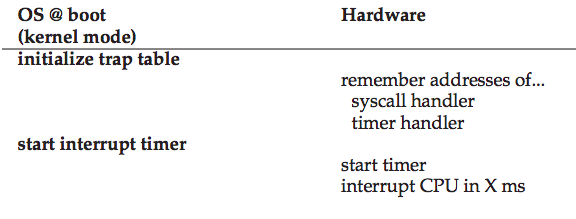
\includegraphics[scale=0.6]{boot}
        \end{figure}
    \end{easylist}

\subsection{Problem 2: Switching Between Processes}
    \begin{easylist}  
    \ListProperties(Hide=100, Hang=true, Progressive=4ex, Style*=--\ , Style2*=$\bullet\ $)
        & How can OS regain control?
        && Because process is running, so OS is not running
        & Cooperative Approach
        && System calls include explicit yield system call, transfering control back to OS
        & Noncooperative Approach
        && Reboot, Timer Interrupt
        & Saving and Restoring Context
        && Scheduler will choose when to switch processes
    \end{easylist}
    \begin{figure}[h]
        \centering
        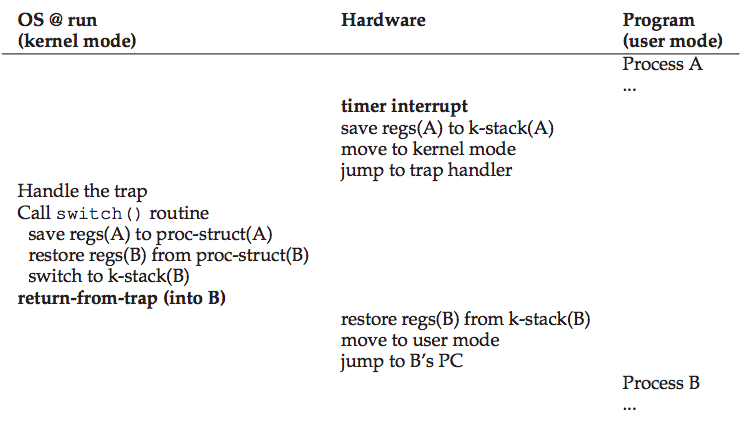
\includegraphics[scale=0.5]{context_switch}
    \end{figure}

\subsection{Worried About Concurrency?}
    \begin{easylist}  
    \ListProperties(Hide=100, Hang=true, Progressive=4ex, Style*=--\ , Style2*=$\bullet\ $)
        & Interrupt during interrupt?
        && Many complex things to do
        && Could disable interrupts (but this might lose interrupts), or locking schemes, etc
    \end{easylist}

\subsection{Summary}
    \begin{easylist}  
    \ListProperties(Hide=100, Hang=true, Progressive=4ex, Style*=--\ , Style2*=$\bullet\ $)
        & Reboot
        && Good technique because restores system to well-tested state
        && OS will 'baby-proof' by only allowing processes to run in restricted mode and with interrupt handlers
    \end{easylist}
%========================================================

%========================================================
\section{L3: Linking and Libraries: Object Modules, Linkage Editing, Libraries}
\subsection{Introduction}
    \begin{easylist}  
    \ListProperties(Hide=100, Hang=true, Progressive=4ex, Style*=--\ , Style2*=$\bullet\ $)
        & Process as fundamental; as executing instance of program
        && Program as one or more files (these are not the executables though)
        && Source must be translated
    \end{easylist}

\subsection{The Software Generation Tool Chain}
    \begin{easylist}  
    \ListProperties(Hide=100, Hang=true, Progressive=4ex, Style*=--\ , Style2*=$\bullet\ $)
        & Source module
        && Editable text in some language like C
        & Relocatable object module
        && Sets of compiled instructions; incomplete programs
        & Library
        && Collection of object modules
        & Load module
        && Complete programs ready to be loaded into memory
        & Compiler
        && Parse source modules; usually generates assembly, may generate pseudo-machine
        & Assembler
        && Object module with mostly machine code
        && Memory addresses of functions, variables may not be filled in
        & Linkage Editor
        && Find all required object modules and resolve all references
        & Program Loader
        && Examines load module, creates virtual space, reads instructions, initializes data values
        && Find and map additional shared libraries
    \end{easylist}

\subsection{Object Modules}
    \begin{easylist}  
    \ListProperties(Hide=100, Hang=true, Progressive=4ex, Style*=--\ , Style2*=$\bullet\ $)
        & Code in multiple files
        && Because more understandable if splitting functionality
        && Many functions are reused, so use external libraries
        & Relocatable object modules are program fragments
        && Incomplete because make references to code in other modules
        && Even the references to other code are only relative 
        & ELF format
        && Header section with types, sizes, and location of other sections
        && Code and data section to be loaded contiguously
        && Symbol table of external symbols
        && Relocation entries describing location of field, width/type of field, symbol table entry
    \end{easylist}

\subsection{Libraries}
    \begin{easylist}  
    \ListProperties(Hide=100, Hang=true, Progressive=4ex, Style*=--\ , Style2*=$\bullet\ $)
        & Reusable, standard functions in libraries 
        && Libraries not always orthogonal and independent
        & Build program by combining object modules and resolving external references 
    \end{easylist}

\subsection{Linkage Editing}
    \begin{easylist}  
    \ListProperties(Hide=100, Hang=true, Progressive=4ex, Style*=--\ , Style2*=$\bullet\ $)
        & Resolution
        && Search libraries to find object modules to resolve external references
        & Loading
        && Lay text and data in single virtual address space
        & Relocation
        && Ensure references correctly reflect chosen address
    \end{easylist}

\subsection{Load Modules}
    \begin{easylist}  
    \ListProperties(Hide=100, Hang=true, Progressive=4ex, Style*=--\ , Style2*=$\bullet\ $)
        & Load module requires no relocation and is complete
        & When loading new module
        && Determine required text and data sizes and locations, allocate segments, read contents, create a stack segment with pointer
        & Load module has symbol table to help determine where exceptions occurred
    \end{easylist}

\subsection{Static vs. Shared Libraries}
    \begin{easylist}  
    \ListProperties(Hide=100, Hang=true, Progressive=4ex, Style*=--\ , Style2*=$\bullet\ $)
        & Static Linking
        && Many copies, so inefficient; also, permenant copy, so don't receive updates
        & Shared Libraries
        && Implementations vary, but one way
        &&& Reserve address for libraries, linkage edit, map with redirection table, etc, more mapping
        && Efficient, but doesn't work for static data because one copy
        && But can be slow to load many libraries, and must know library name at loadtime
    \end{easylist}

\subsection{Dynamically Loaded Libraries}
    \begin{easylist}  
    \ListProperties(Hide=100, Hang=true, Progressive=4ex, Style*=--\ , Style2*=$\bullet\ $)
        & DLL loaded once needed
        && Choose and load library, binds, use library, unload
        && Resource efficient because can unload
        & Implicitly Loaded Dynamically Loadable Libraries
        && Another implementation of DLL with different pros/cons
    \end{easylist}
%========================================================

%========================================================
\section{L3: Linkage Conventions: Stack Frames and Linkage Conventions}
\subsection{Introduction}
    \begin{easylist}  
    \ListProperties(Hide=100, Hang=true, Progressive=4ex, Style*=--\ , Style2*=$\bullet\ $)
        & What is the state of computation and how can it be saved?
        & What is the mechanism of requesting and receiving services?
    \end{easylist}

\subsection{The Stack Model of Programming Languages}
    \begin{easylist}  
    \ListProperties(Hide=100, Hang=true, Progressive=4ex, Style*=--\ , Style2*=$\bullet\ $)
        & Procedure-local variables
        && Stored on a LIFO stack
        && New call frames pushed onto stack when procedure called; old frames popped when procedure reutrns
        && Long-lived resources on heap, not stack
    \end{easylist}

\subsection{Subroutine Linkage Conventions}
    \begin{easylist}  
    \ListProperties(Hide=100, Hang=true, Progressive=4ex, Style*=--\ , Style2*=$\bullet\ $)
        & X86 Subroutine Linkage
        && Pass parameters to be called by routine
        && Save return address and transfer control to entry
        && Save content of non-volatile registers
        && Allocate space for local variables
        & X86 Return Process
        && Return value to where routine expects it
        && Pop local storage
        && Restore registers
        && Subroutine transfer control to return address
        & Responsibilities split between caller and callee
        & Saving and restoring state of procedure is mostly a matter of stack frame and registers
    \end{easylist}

\subsection{Traps and Interrupts}
    \begin{easylist}  
    \ListProperties(Hide=100, Hang=true, Progressive=4ex, Style*=--\ , Style2*=$\bullet\ $)
        & Procedure call vs Trap/Interrupt
        && Procedure requested by running software and expects result; linkage conventions under software control
        && After trap/interrupt, should restore state
        & How
        && Number associated with every interrupt/exception, maps to PS/PC
        && Push new program counter and program status (from interrupt/trap vector table) onto CPU stack
        && Resume execution at new PC
        && First level handler
        &&& Save general registers on stack
        &&& Choose second level handler based on info from interrupt/trap
        && Second level handler (procedure call)
        &&& Deal with interrupt/exception
        &&& Return to first level handler 
        &&&& Restore saved registers and return-from-interrupt/trap
        && CPU realoads PC/PS and resumes execution
        & Stacking/unstacking interrupt/trap is 100x+ slower than procedure call
    \end{easylist}
\clearpage
%========================================================

%========================================================
\section{L4: Arpaci-Dusseau Chapter 7: Scheduling: Introduction}
\subsection{Workload Assumptions}
    \begin{easylist}  
    \ListProperties(Hide=100, Hang=true, Progressive=4ex, Style*=--\ , Style2*=$\bullet\ $)
        & Workload as the processes running in the system
        & Fully-operational scheduling discipline
        && Assume each job runs for same amount of time, arrives at same time, once started will run to completion, only uses CPU, run-time length is known
    \end{easylist}

\subsection{Scheduling Metrics}
    \begin{easylist}  
    \ListProperties(Hide=100, Hang=true, Progressive=4ex, Style*=--\ , Style2*=$\bullet\ $)
        & Scheduling metric is something we can measure is useful for scheduling
        && $Turnaround_{time}: Time_{completion} - Time_{arrival}$
        & Performance and Fairness often at odds with each other
        && Fairness measured by Jain's Fairness Index
    \end{easylist}

\subsection{First In, First Out (FIFO)}
    \begin{easylist}  
    \ListProperties(Hide=100, Hang=true, Progressive=4ex, Style*=--\ , Style2*=$\bullet\ $)
        & Properties of FIFO
        && Simple and easy to implement while working well based on assumptions
        & Convoy Effect
        && FIFO fails if few high-resource consumers are ahead of low-resource consumers
    \end{easylist}

\subsection{Shortest Job First (SJF)}
    \begin{easylist}  
    \ListProperties(Hide=100, Hang=true, Progressive=4ex, Style*=--\ , Style2*=$\bullet\ $)
        & SJF is optimal given the assumptions
        && But fails if relaxes arrival-time assumption
        && A long process may start, then a short process comes in
    \end{easylist}

\subsection{Shortest Time-to-Completion First (STCF)}
    \begin{easylist}  
    \ListProperties(Hide=100, Hang=true, Progressive=4ex, Style*=--\ , Style2*=$\bullet\ $)
        & Preemptive schedulers will context switch to run another process
        && Non-preemptive schedulers run jobs to completion before considering another
        && SJF is nonpreemptive
        & Shortest time-to-completion (STCF) also known as Preemptive shortest job first (PSJF)
        && Anytime a new job arrives, determine which job has shortest time remaining, and runs that one
    \end{easylist}

\subsection{A New Metric: Response Time}
    \begin{easylist}  
    \ListProperties(Hide=100, Hang=true, Progressive=4ex, Style*=--\ , Style2*=$\bullet\ $)
        & $T_{response}: T_{firstrun} - T_{arrival}$
        & STCF is especially bad for optimizing response time
    \end{easylist}

\subsection{Round Robin}
    \begin{easylist}  
    \ListProperties(Hide=100, Hang=true, Progressive=4ex, Style*=--\ , Style2*=$\bullet\ $)
        & RR (time-slicing) runs job for a time slice (scheduling quantum) before switching to next
        && Length of time slice is essential; if long, then long $T_{response}$; if short, context switching dominates
        && Must choose a length of time which will amortize the cost well
        && Also must consider cost of flushing CPU caches, TLBs, branch predictors, chip hardware
        & Performs extremely poorly wrt turnaround time
        && Most fair policies (evenly distribute) are like this
    \end{easylist}

\subsection{Incorporating I/O}
    \begin{easylist}  
    \ListProperties(Hide=100, Hang=true, Progressive=4ex, Style*=--\ , Style2*=$\bullet\ $)
        & Overlap leads to higher utilization and better performance
        && Use for IO, messages, etc
        & Overlap CPU when one process requires IO
        && While IO for process A, run process B on CPU (because A is blocked)
    \end{easylist}

\subsection{No More Oracle/Summary}
    \begin{easylist}  
    \ListProperties(Hide=100, Hang=true, Progressive=4ex, Style*=--\ , Style2*=$\bullet\ $)
        & Assumption of known run-time length is highly invalid
        & Shortest job remaining optimizes turnaround time
        & Alternating between jobs optimizes response time
        & Looking ahead
        && Multi-level feedback: Using past events to predict future
    \end{easylist}
%========================================================

%========================================================
\section{L4: Arpaci-Dusseau Chapter 8: Scheduling: The Multi-Level Feedback Queue}
\subsection{MLFQ: Basic Rules}
    \begin{easylist}  
    \ListProperties(Hide=100, Hang=true, Progressive=4ex, Style*=--\ , Style2*=$\bullet\ $)
        & MFLQ has a number of distinct queues with different priority levels
        & If priority(A) $<$ priority(B), A runs
        & If priority(A) == priority(B), A and B run in RR
        & Vary priority based on observed behavior
    \end{easylist}

\subsection{Attempt 1: How To Change Priority}
    \begin{easylist}  
    \ListProperties(Hide=100, Hang=true, Progressive=4ex, Style*=--\ , Style2*=$\bullet\ $)
        & When job enters, has highest priority
        & If job uses entire time slice, priority is reduced
        & If job gives up CPU early, priority remains the same
        & Assume jobs are short so that it will either complete or move down in priority
        & Starvation
        && If there are too many interactive (IO) jobs, then longer processes with low priority will never run
        & Gaming the scheduler
        && Could write program to use less than entire timeslice, to always keep highest priority
        & Changing Behavior
        && Program may become interactive after computations, so needs higher priority
    \end{easylist}

\subsection{Attempt 2: The Priority Boost}
    \begin{easylist}  
    \ListProperties(Hide=100, Hang=true, Progressive=4ex, Style*=--\ , Style2*=$\bullet\ $)
        & Boost all processes to top priority after a certain time length
        & Difficult to know correct value for these voo-doo constant parameters (refer to Ousterhout’s Law)
    \end{easylist}

\subsection{Attempt 3: Better Accounting}
    \begin{easylist}  
    \ListProperties(Hide=100, Hang=true, Progressive=4ex, Style*=--\ , Style2*=$\bullet\ $)
        & Account CPU time (Anti-gaming method)
        && Once job uses up time allotment on given level, priority is reduced
    \end{easylist}

\subsection{Tuning MLFQ And Other Issues}
    \begin{easylist}  
    \ListProperties(Hide=100, Hang=true, Progressive=4ex, Style*=--\ , Style2*=$\bullet\ $)
        & Difficult to find correct parameters
        && High-priority queue contains interactive processes and run for short timeslices (20ms)
        && Low-priority queue contains long-running processes and so run for longer timeslices (up to a few hundred ms)
        && Many queues, like 60
        && Priorities boosted every second or so
        & Other schedulers use mathematical formulas to calculate priority (decay-usage)
        & Even may offer advice to scheduler using Linux's nice program
    \end{easylist}

\subsection{MLFQ: Summary}
    \begin{easylist}  
    \ListProperties(Hide=100, Hang=true, Progressive=4ex, Style*=--\ , Style2*=$\bullet\ $)
        & Multiple levels of queues with feedback to determine priority
        & Rules
        && If priority(A) $>$ priority(B), A runs
        && If priority(A) = priority(B), A and B run in RR
        && When a job enters the system, has highest priority
        && When a job uses entire time allotment at a given level, its priority is reduced
        && After some time period S, move all the jobs in the system to the topmost queue
    \end{easylist}
%========================================================

%========================================================
\section{L4: Real Time Scheduling}
\subsection{What are Real-Time Systems}
    \begin{easylist}  
    \ListProperties(Hide=100, Hang=true, Progressive=4ex, Style*=--\ , Style2*=$\bullet\ $)
        & Priority scheduling is best effort
        && Sometimes need more than just best effort (space shuttle reentry, data, assembly line, media players)
        & Traditonal vs Real-time systems
        && Turn-around time, fairness, response time for traditional
        && Timeliness may be ms/day of accumulated tardiness
        && Predictability is deviation in delivered timeliness
        && Feasibility is whether possible to meet requirements
        && Hard real-time is a requirement to run specifiy tasks at specified intervals 
        && Soft real-time requires good response time, at the cost of degraded performance or recoverable failure
        & Real-time systems 
        && May know length of jobs/priorities, and starvation of certain jobs may be acceptable
    \end{easylist}

\subsection{Real-Time Scheduling Algorithms}
    \begin{easylist}  
    \ListProperties(Hide=100, Hang=true, Progressive=4ex, Style*=--\ , Style2*=$\bullet\ $)
        & Static scheduling
        && May be possible to define fixed schedule if know all tasks to run and expected completion time
        & Dynamic Scheduling for changing workloads
        && Questions of how to choose next task and how to deal with overload
        & If high enough frequency of work, may just work for sufficiently-light loaded systems
    \end{easylist}

\subsection{Real-Time and Linux}
    \begin{easylist}  
    \ListProperties(Hide=100, Hang=true, Progressive=4ex, Style*=--\ , Style2*=$\bullet\ $)
        & Linux was not designed as embedded or real-time system
        && Supports a real-time scheduler sched\_setscheduler, but still does not have same level of response-times
        & Windows believes in general throughput not deadlines, and is bad for critical real-time operations 
    \end{easylist}
\clearpage
%========================================================

%========================================================
\section{L5: Arpaci-Dusseau Chapter 12: A Dialogue on Memory Virtualization}
\subsection{Overview}
    \begin{easylist}  
    \ListProperties(Hide=100, Hang=true, Progressive=4ex, Style*=--\ , Style2*=$\bullet\ $)
        & Every address generated by a user program is a virtual address
        && Large contiguous address space is easier to work with than small crowded space
        && Isolation and protetion are also important in preventing processes each other's memory
    \end{easylist}
%========================================================

%========================================================
\section{L5: Arpaci-Dusseau Chapter 13: The Abstraction: Address Spaces}
\subsection{Early Systems}
    \begin{easylist}  
    \ListProperties(Hide=100, Hang=true, Progressive=4ex, Style*=--\ , Style2*=$\bullet\ $)
        & OS as set of routines (a library)
        & Program in physical memory used rest of space
    \end{easylist}

\subsection{Multiprogramming and Time Sharing}
    \begin{easylist}  
    \ListProperties(Hide=100, Hang=true, Progressive=4ex, Style*=--\ , Style2*=$\bullet\ $)
        & Multiprogramming
        && Multiple processes ready to run at a given time with OS switching between them
        && Increases utilization of CPU; increased efficiency of CPU is very relevant bc so expensive
        & Timesharing and interactivity
        && Long program-debug cycles bad for programmers
        && Giving all programs full access to memory is not safe
    \end{easylist}

\subsection{The Address Space}
    \begin{easylist}  
    \ListProperties(Hide=100, Hang=true, Progressive=4ex, Style*=--\ , Style2*=$\bullet\ $)
        & Address space is easy to use abstraction of physical memory
        && Contains code, stack, heap
        && Every program thinks it had very large address space, even though it doesn't
    \end{easylist}

\subsection{Goals}
    \begin{easylist}  
    \ListProperties(Hide=100, Hang=true, Progressive=4ex, Style*=--\ , Style2*=$\bullet\ $)
        & Transparency
        && Cannot tell that memory is virtual
        & Efficiency
        && OS should make virtualization efficient wrt time and space, relying on hardware for this
        & Protection
        && Isolate process memory from each other
    \end{easylist}
%========================================================

%========================================================
\section{L5: Arpaci-Dusseau Chapter 14: Interlude: Memory API}
\subsection{Types of Memory}
    \begin{easylist}  
    \ListProperties(Hide=100, Hang=true, Progressive=4ex, Style*=--\ , Style2*=$\bullet\ $)
        & Stack
        && Automatic memory is managed implicitly by compiler
        & Heap
        && Long lived memory where allocations and deallocations handled by programmer
    \end{easylist}

\subsection{The malloc()/free() Call}
    \begin{easylist}  
    \ListProperties(Hide=100, Hang=true, Progressive=4ex, Style*=--\ , Style2*=$\bullet\ $)
        & double *d = (double *) malloc(sizeof(double));
        & free(d); // prevents memory leaks
    \end{easylist}

\subsection{Common Errors}
    \begin{easylist}  
    \ListProperties(Hide=100, Hang=true, Progressive=4ex, Style*=--\ , Style2*=$\bullet\ $)
        & Modern languages have automatic memory-management or a garbage collector because people don't free
        & Seg fault if you forget to allocate
        & Buffer overflow if not enough allocated space
        & Dangling pointer if you free memory before finished using it
        & Double freeing memory is undefined
        & Incorrect use of free (passing it things other than pointer from malloc) is dangerous
        & Use Valground and Purify to find memory leaks
    \end{easylist}

\subsection{Underlying OS Support}
    \begin{easylist}  
    \ListProperties(Hide=100, Hang=true, Progressive=4ex, Style*=--\ , Style2*=$\bullet\ $)
        & Break is the location at the end of the heap
        && System call brk is used to increase/decrease size of heap
    \end{easylist}
%========================================================

%========================================================
\section{L5: Arpaci-Dusseau Chapter 17: Free-Space Management}
\subsection{Assumptions}
    \begin{easylist}  
    \ListProperties(Hide=100, Hang=true, Progressive=4ex, Style*=--\ , Style2*=$\bullet\ $)
       & Free list manages the heap; contains references to all the free chunks in the region
       & External fragmentation
       && Have enough space, but not contiguous, so can't malloc
       & Internal fragmentation 
       && Gives memory larger than requested, which remains unused
    \end{easylist}

\subsection{Low-level Mechanisms}
    \begin{easylist}  
    \ListProperties(Hide=100, Hang=true, Progressive=4ex, Style*=--\ , Style2*=$\bullet\ $)
        & Splitting and Coalescing
        && Split free chunk in two, returning first to the caller
        && Coalesces adjacent free memory together, forming a single larger free chunk
        & Header of allocated memory
        && Contains size of region and magic number to speed up deallocation
        & Embedding free list
        && Build free list inside the free space itslf
        && Nodes with size and next pointer
        & Growing heap
        && Just give up and return NULL
        && Or call sbrk system call to OS to grow heap
    \end{easylist}

\subsection{Basic Strategies}
    \begin{easylist}  
    \ListProperties(Hide=100, Hang=true, Progressive=4ex, Style*=--\ , Style2*=$\bullet\ $)
        & Best fit
        && Return smallest chunk that is equal or larger than the requested size
        && Requires linear search
        & Worst fit
        && Find largest chunk, split it, return requested size
        && Requires linear search
        & First fit
        && Returns first block big enough
        && Faster because no exhaustive search
        & Next fit
        && Returns first block big enough starting from previous location
        && Spreads searches through free space more uniformly 
    \end{easylist}

\subsection{Other Approaches}
    \begin{easylist}  
    \ListProperties(Hide=100, Hang=true, Progressive=4ex, Style*=--\ , Style2*=$\bullet\ $)
        & Segregated Lists
        && Keep separated list to manage all objects of that size
        && Hard to determine much memory to dedicate to that list
        & Slab allocator by Jeff Bonwick
        && Object caches for kernel objects 
        && Each object cache are segregated free lists
        && Requests slabs of memory from general allocator, when running low
        & Binary buddy Allocation
        && Big space of $2^N$
        && Suffers from internal fragmentation but can recursively coalesce 
    \end{easylist}
%========================================================

%========================================================
\section{L5: Garbage Collection and Defragmentation}
\subsection{Garbage Collection}
    \begin{easylist}  
    \ListProperties(Hide=100, Hang=true, Progressive=4ex, Style*=--\ , Style2*=$\bullet\ $)
        & Allocated resources are freed through explicit/implicit action by client
        && close(2), free(3), delete operator, returning from a C/C++ subroutin, exit(2)
        & If shared by multiple concurrent clients
        && Free only if reference count is zero (don't free if others are still using it, just decrement the reference count)
        & Garbage Collection
        && Analyzes allocated resources to determine which are still in use
        && Data structures assoc with resource references are designed to be easily enumerated to enable the scan for accessible resources
        && Comes at a performance cost
    \end{easylist}

\subsection{Defragmentation}
    \begin{easylist}  
    \ListProperties(Hide=100, Hang=true, Progressive=4ex, Style*=--\ , Style2*=$\bullet\ $)
        & Shards of free memory are not useful
        && Coalescing is only useful if adjacent memory free at same time
        & Defragmentation
        && Changes which resources are still allocated
        & Flash management
        && NAND Flash is a pseudo-Write-Once-Read-Many medium
        && Identify large (64MB) block with many 4KB blocks not in use
        && Move all in use blocks and update resource allocation map
        && Erase large block and add 4KB blocks to free list
        & Disk Space Allocation
        && Choose region to create contiguous free space
        && For each file in that region, move it elsewhere
        && Coalesce all that free memory
        && Move set of files into that region
        && Repeat until all files and free space is contiguous
        & Internal fragmentation is like rust, it never sleeps
        && Defragmentation used to be run periodically, now is run continuously
        & Conclusions
        && If using garbage collection, must make all resources discoverable, how to trigger scans, prevent race conditions with application
        && Must not disrupt running applications when using defragmentation
    \end{easylist}
\clearpage
%========================================================

%========================================================
\section{L6: Arpaci-Dusseau Chapter 18: Paging: Introduction}
\subsection{A Simple Example And Overview}
    \begin{easylist}  
    \ListProperties(Hide=100, Hang=true, Progressive=4ex, Style*=--\ , Style2*=$\bullet\ $)
        & Paging
        && Divide process address space into fixed-sized units
        && View memory as fixed-sized page frames
        & Free list
        && OS may hold list of free pages
        & Page table is a per process data structure
        && Stores address translations for virtual pages so we know where it is in physical memory
        & Virtual address [VPN, OFFSET]
        && Virtual page number (VPN) indexes page table to find physical frame/page number (PFN/PPN)
        && Translate VPN to PPN then load from memory
        && Offset determines which byte within page
    \end{easylist}

\subsection{Where Are Page Tables Stored?}
    \begin{easylist}  
    \ListProperties(Hide=100, Hang=true, Progressive=4ex, Style*=--\ , Style2*=$\bullet\ $)
        & Page table entry
        && Holds physical translation 
        && If roughly 4 bytes per PTE, page tables would be big
        && Problem bc page table per process
        & Stored somewhere in memory
    \end{easylist}

\subsection{What’s Actually In The Page Table?}
    \begin{easylist}  
    \ListProperties(Hide=100, Hang=true, Progressive=4ex, Style*=--\ , Style2*=$\bullet\ $)
        & Linear Page Table
        && Index array by VPN to look up PTE and to find physical frame number (PFN)
        && Valid bit indicates if memory is valid (traps if invalid)
        && Proction bit indicates whether page can be read/written/executed (trap if bad access)
        && Present bit indicates whether page is in memory or disk (if it has been swapped out)
        && Dirty bit indicates if page has been modified since brought into memory
        && Reference/aceess bit indicates if page has been accessed (to determine which pages are popular; used for page replacement) 
    \end{easylist}

\subsection{Paging: Also Too Slow}
    \begin{easylist}  
    \ListProperties(Hide=100, Hang=true, Progressive=4ex, Style*=--\ , Style2*=$\bullet\ $)
        & Must translate virtual address
        && VPN = (Virtual address \& $VPN_{MASK}$) $>>$ SHIFT
        && PTEaddr = Page table base address + VPN * sizeof(PTE)
        && Offset = Virtual address \& $OFFSET_{MASK}$
        && PhysAddr = (PFN $<<$ SHIFT) | Offset
    \end{easylist}
%========================================================

%========================================================
\section{L6: Arpaci-Dusseau Chapter 19: Paging: Faster Translations (TLBs)}
\subsection{TLB Basic Algorithm}
    \begin{easylist}  
    \ListProperties(Hide=100, Hang=true, Progressive=4ex, Style*=--\ , Style2*=$\bullet\ $)
        & TLB
        && Bc chopped address space into many fixed-sized units, paging requires a lot of memory to map addresses 
        && This mapping memory is also stored in physical memory, which would require an additional memory lookup to read
        && Instead, use a TLB, which is an address translation cache, to hold popular virtual-to-physical translations
        & TLB Hit/miss
        && If virtual page number (VPN) from virtual address (VA) is inside the TLB (translation lookaside buffer), then have TLB hit and may extract the page frame number (PFN)
        && If VPN from VA is not inside TLB, then have TLB miss and must access page table (in memory) to find translation, update TLB, then restart lookup into TLB
    \end{easylist}

\subsection{Example: Accessing An Array}
    \begin{easylist}  
    \ListProperties(Hide=100, Hang=true, Progressive=4ex, Style*=--\ , Style2*=$\bullet\ $)
        & Start with a miss, then multiple hits
        && Rely on spatial locality for first pass
        && Rely on temporal locality for second pass
        & Caching is fundamental
        && Temporal and spatial locality are necessary
        && Can't make caches large because physics says large cache is slow    
    \end{easylist}

\subsection{Who Handles The TLB Miss?}
    \begin{easylist}  
    \ListProperties(Hide=100, Hang=true, Progressive=4ex, Style*=--\ , Style2*=$\bullet\ $)
        & Hardware
        && Use page table base register to walk page table and find PTE
        & Software
        && Hardware raises exception, pauses instructions, privilege raises to kernel mode, jumps to trap handler
        & Infinite TLB misses
        && If is a problem, keep TLB miss handlers in physical memory (unmapped) so it will always be a hit
        & RISC vs CISC (Aside)
        && Complex has more and more powerful instructions
        && Reduced has fewer and simpler primitives
    \end{easylist}

\subsection{TLB Contents: What’s In There?}
    \begin{easylist}  
    \ListProperties(Hide=100, Hang=true, Progressive=4ex, Style*=--\ , Style2*=$\bullet\ $)
        & Fully associative means a given translation can be anywhere in the TLB
        & VPN  | PFN | other bits
        && Other bits include valid bit, protection bits (regarding w/r/x), address space identifier, dirty bit, etc
    \end{easylist}

\subsection{TLB Issue: Context Switches}
    \begin{easylist}  
    \ListProperties(Hide=100, Hang=true, Progressive=4ex, Style*=--\ , Style2*=$\bullet\ $)
        & Fully associative means a given translation can be anywhere in the TLB
        & VPN  | PFN | other bits
        && Other bits include valid bit, protection bits (regarding w/r/x), address space identifier, dirty bit, etc
        && Could flush TLB on context switch, or could use address space identifier
    \end{easylist}

\subsection{Issue: Replacement Policy}
    \begin{easylist}  
    \ListProperties(Hide=100, Hang=true, Progressive=4ex, Style*=--\ , Style2*=$\bullet\ $)
        & LRU Replacement Policy
        && Least recently used, but usually can't actually do this, so vaguely do LRU
    \end{easylist}
%========================================================

%========================================================
\section{L6: Arpaci-Dusseau Chapter 21: Beyond Physical Memory: Mechanisms}
\subsection{Swap Space}
    \begin{easylist}  
    \ListProperties(Hide=100, Hang=true, Progressive=4ex, Style*=--\ , Style2*=$\bullet\ $)
        & Swap Space
        && Use hard disk drive as storage
        && Reserved space on disk for moving pages back and forth
    \end{easylist}

\subsection{The Present Bit}
    \begin{easylist}  
    \ListProperties(Hide=100, Hang=true, Progressive=4ex, Style*=--\ , Style2*=$\bullet\ $)
        & Extract VPN from VA, check for TLB hit and produce PA if possible
        && Otherwise, receive TLB miss and go to memory through page table base register to find PTE
        & Present bit
        && Set to one if page is in physical memory
        && Otherwise, is not in physical memory and is a page fault
        && OS invoked to service page fault, so page-fault handler runs
    \end{easylist}

\subsection{The Page Fault}
    \begin{easylist}  
    \ListProperties(Hide=100, Hang=true, Progressive=4ex, Style*=--\ , Style2*=$\bullet\ $)
        & OS page-fault handler
        && Hardware does not do it because hardware does not know enough about swap space, I/O, etc
        && OS looks in PTE to find address and request it from disk
        && Process is blocked during this, so run another process
    \end{easylist}

\subsection{What If Memory Is Full?}
    \begin{easylist}  
    \ListProperties(Hide=100, Hang=true, Progressive=4ex, Style*=--\ , Style2*=$\bullet\ $)
        & Page-replacement Policy
        && Page in from swap space; Page out from memory
        && Replace if memory is full
        && 10k-100k times slower if poor page-replacement policy
    \end{easylist}

\subsection{Page Fault Control Flow}
    \begin{easylist}  
    \ListProperties(Hide=100, Hang=true, Progressive=4ex, Style*=--\ , Style2*=$\bullet\ $)
        & If TLB miss
        && If invalid, OS trap handle terminates process
        && If not present, run page fault handler
        &&& Find physical frame for soon-to-be-faulted-in page
        &&& Run replacement alg if necessary
        &&& I/O request page from swap space
        &&& Retry for TLB miss, then retry for TLB hit
        && If present and valid, grab PFN from PTE and retry
    \end{easylist}

\subsection{When Replacements Really Occur}
    \begin{easylist}  
    \ListProperties(Hide=100, Hang=true, Progressive=4ex, Style*=--\ , Style2*=$\bullet\ $)
        & Swap daemon
        && If fewer pages than the low watermark, then background thread evicts pages 
        && Continues evicting pages until the high watermark
        && Then goes back to sleep and waits
        & Clustering
        && Clustering/grouping these pages to swap partition increases efficiency because it reduces disk seek and rotational overheads
        & Background work
        && Do work in background (buffered disk writes, etc) because it is more efficient and makes better use of idle time 
    \end{easylist}
%========================================================

%========================================================
\section{L6: Arpaci-Dusseau Chapter 22: Beyond Physical Memory: Policies}
\subsection{Cache Management}
    \begin{easylist}  
    \ListProperties(Hide=100, Hang=true, Progressive=4ex, Style*=--\ , Style2*=$\bullet\ $)
        & Minimize cache misses because a single miss will make it very slow
        && Average memory access time (AMAT) $= T_M + (P_{miss} * T_D)$
    \end{easylist}

\subsection{The Optimal Replacement Policy}
    \begin{easylist}  
    \ListProperties(Hide=100, Hang=true, Progressive=4ex, Style*=--\ , Style2*=$\bullet\ $)
        & Farthest in the future
        && Is optimal
        && Use this as a reference point, something to compare our algorithms against
        & Types of misses
        && Cold-start miss is compulsory because cache is empty
        && Capacity miss is because cache ran out of space
        && Conflict miss is because of hardware limits on where items can be placed in a hardware cache (not a problem for OS page cache)
    \end{easylist}

\subsection{Replacement Policies}
    \begin{easylist}  
    \ListProperties(Hide=100, Hang=true, Progressive=4ex, Style*=--\ , Style2*=$\bullet\ $)
        & FIFO
        && Performs quite terribly, but is simple to implement
        && Belady's Anomaly: FIFO performs even worse on larger cache than on smaller cache
        & Random
        && Can work
        & Least-Frequently-Used (LFU)/Least-Recently-Used (LRU)
        && Rely on locality and do what their names say
        & Most-Frequently-Used (MFU)/Most-Recently-Used (MRU)
        && Exist and do not work well
        & Workload examples
        && FIFO doesn't do well, random can do well, LRU does fairly well
    \end{easylist}

\subsection{Implementing LRU}
    \begin{easylist}  
    \ListProperties(Hide=100, Hang=true, Progressive=4ex, Style*=--\ , Style2*=$\bullet\ $)
        & True LRU is expensive
        && Finding truly least-recently-used page is prohibitively time-consuming
        & Approximate LRU using Clock algorithm
        && Whenever page is referenced, use bit is set
        && Clock hand points to some page, if bit is set, unsets it and checks next
        && If bit is unset, replaces it
    \end{easylist}

\subsection{Considering Dirty Pages}
    \begin{easylist}  
    \ListProperties(Hide=100, Hang=true, Progressive=4ex, Style*=--\ , Style2*=$\bullet\ $)
        & If page is dirty (set dirty bit), then must be written back to disk if we want to evict it
        && Prefer to evict clean pages
    \end{easylist}

\subsection{Other VM Policies}
    \begin{easylist}  
    \ListProperties(Hide=100, Hang=true, Progressive=4ex, Style*=--\ , Style2*=$\bullet\ $)
        & Demand Paging
        && Bring page into memory only 'on demand'
        && Opposite of prefetching memory
        & Clustering/Grouping of writes
        && Write many things at same time because of how disk drive works
    \end{easylist}

\subsection{Thrashing}
    \begin{easylist}  
    \ListProperties(Hide=100, Hang=true, Progressive=4ex, Style*=--\ , Style2*=$\bullet\ $)
        & If memory is just oversubscribed
        && Then will constantly page and thrash
        & Admission control
        && Decide to not run some processes, so that we may do well on the remaining processes
        & Out-of-memory killer
        && Will choose a memory-intensive process and kill it
    \end{easylist}
%========================================================

%========================================================
\section{L6: Working Sets}
\subsection{LRU is not enough}
    \begin{easylist}  
    \ListProperties(Hide=100, Hang=true, Progressive=4ex, Style*=--\ , Style2*=$\bullet\ $)
        & Global LRU
        && Most-recently used page is from current process and will not run for a while
        && Least-recently used page is from old process about to run
    \end{easylist}

\subsection{The concept of a Working Set}
    \begin{easylist}  
    \ListProperties(Hide=100, Hang=true, Progressive=4ex, Style*=--\ , Style2*=$\bullet\ $)
        & Is the set of pages for a given process
        && Increasing the number of pages makes little difference in performance, but decreasing makes a difference
        & Different computations require different sizes, getting the number correct will minimize page faults and maximize throughput
    \end{easylist}

\subsection{Implementing Working Set replacement}
    \begin{easylist}  
    \ListProperties(Hide=100, Hang=true, Progressive=4ex, Style*=--\ , Style2*=$\bullet\ $)
        & More information recorded about pages
        && Associated with owning process
        && Accumulated CPU time 
        && Last referenced time
        && Target age parameter 
        & Age decisions are made on the basis of accumulated CPU time
        && Page ages if owner runs without them
        && Pages younger than a target age are preferrably not replaced
        && Give pages older than target age away
    \end{easylist}

\subsection{Dynamic Equilibrium to the rescue}
    \begin{easylist}  
    \ListProperties(Hide=100, Hang=true, Progressive=4ex, Style*=--\ , Style2*=$\bullet\ $)
        & Page stealing algorithm
        && Every process is continuously losing and stealing pages
        && Processes that reference more pages more often will accumulate larger working sets while others will find their set reduced
        && Working sets adjust automatically
    \end{easylist}
\clearpage
%========================================================

%========================================================
\section{L7: Arpaci-Dusseau Chapter 25: A Dialogue on Concurrency}
\subsection{Dialogue}
    \begin{easylist}  
    \ListProperties(Hide=100, Hang=true, Progressive=4ex, Style*=--\ , Style2*=$\bullet\ $)
        & Multi-threaded applications
        && Threads access memory; we don't want multiple threads to access memory at same time
        && OS supports primitives such as locks and condition variables
    \end{easylist}
%========================================================

%========================================================
\section{L7: Arpaci-Dusseau Chapter 26: Concurrency: An Introduction}
\subsection{Introduction}
    \begin{easylist}  
    \ListProperties(Hide=100, Hang=true, Progressive=4ex, Style*=--\ , Style2*=$\bullet\ $)
        & Context switch
        && Save state (program counter, registers) to thread control block
        && Address space stays the same, so page table does not need to be switched
        & Multiple stacks in address space if multiple threads
        & Thread-local storage
        && Stack of that thread
    \end{easylist}

\subsection{Why Use Threads?}
    \begin{easylist}  
    \ListProperties(Hide=100, Hang=true, Progressive=4ex, Style*=--\ , Style2*=$\bullet\ $)
        & Used threads to exploit parallelism
        && If single processor, then not relevant
        && Otherwise, parallelize and used thread per CPU
        & Use threads to do someting when blocked program
        && Instead of waiting for IO, just switch to another thread and do things
        & Choose process for logically separate tasks with little sharing of data structures
    \end{easylist}

\subsection{An Example: Thread Creation}
    \begin{easylist}  
    \ListProperties(Hide=100, Hang=true, Progressive=4ex, Style*=--\ , Style2*=$\bullet\ $)
        & Use pthreads
        & Will run in different order according to scheduler
        & May not be deterministic
    \end{easylist}

\subsection{The Heart Of The Problem: Uncontrolled Scheduling}
    \begin{easylist}  
    \ListProperties(Hide=100, Hang=true, Progressive=4ex, Style*=--\ , Style2*=$\bullet\ $)
        & Race condition
        && Execution depends on timing execution of code (indeterminate)
        & Critical section
        && Multiple threads executing code resulting in race condition
        & Mutual exclusion
        && If one thread executing inside critical section, others will be prevented
    \end{easylist}

\subsection{The Wish For Atomicity}
    \begin{easylist}  
    \ListProperties(Hide=100, Hang=true, Progressive=4ex, Style*=--\ , Style2*=$\bullet\ $)
        & Atomic (all or nothing)
        && Don't just have atomic instructions for all because too many instrucions
        & Synchronization primitives
        && General set of instructions to control multi-threaded programs
    \end{easylist}
%========================================================

%========================================================
\section{L7: Arpaci-Dusseau Chapter 27: Interlude: Thread API}
\subsection{Threads}
    \begin{easylist}  
    \ListProperties(Hide=100, Hang=true, Progressive=4ex, Style*=--\ , Style2*=$\bullet\ $)
        & Use pthreat\_create to create new thread
        & Use pthread\_join to wait for thread to complete
        & Use pthread\_mutex\_lock and pthread\_mutex\_unlock to provide mutual exclusion to critical sections via locks
        && Need to properly initialize and check that lock/unlock actually succeed
        & Condition variables
        && Enables thread to wait until particular condition occurs
        && Needs lock and condition
        && Sleeps until other thread signals
        & Spinlock
        && Wait in loop until lock available, consuming CPU cycles
    \end{easylist}
%========================================================

%========================================================
\section{L7: User-Mode Thread Implementation}
\subsection{Introduction}
    \begin{easylist}  
    \ListProperties(Hide=100, Hang=true, Progressive=4ex, Style*=--\ , Style2*=$\bullet\ $)
        & Threads are independent schedulable unit of execution
        && Runs within address space of process
        && Has access to system resources from process
        && Has own registers and stack
    \end{easylist}

\subsection{User/Kernel}
    \begin{easylist}  
    \ListProperties(Hide=100, Hang=true, Progressive=4ex, Style*=--\ , Style2*=$\bullet\ $)
        & User-level thread done without OS
        && Allocates memory, dispathes thread, sleeps, exits, free memory
        && If system call blocks, entire process blocks
        && Cannot exploit multi-processors
        & Kernel implemented threads
        && Exploits multi-processors and switches between threads when one blocks
    \end{easylist}
\subsection{User/Kernel}
    \begin{easylist}  
    \ListProperties(Hide=100, Hang=true, Progressive=4ex, Style*=--\ , Style2*=$\bullet\ $)
        & Non-preemptive scheduling
        && User-mode threads are more efficient than kernel for contex-switches
        & Preemptive scheduling
        && Allowing OS to schedule is better than setting alarms and signals
    \end{easylist}
%========================================================

%========================================================
\section{L7: Inter-Process Communication}
\subsection{Introduction}
    \begin{easylist}  
    \ListProperties(Hide=100, Hang=true, Progressive=4ex, Style*=--\ , Style2*=$\bullet\ $)
        & coordination of operations with other processes
        && synchronization (e.g. mutexes and condition variables)
        && the exchange of signals (e.g. kill(2))
        && control operations (e.g. fork(2), wait(2), ptrace(2))
        & the exchange of data between processes:
        && uni-directional/bi-directional 
    \end{easylist}

\subsection{Simple Uni-Directional Byte Streams}
    \begin{easylist}  
    \ListProperties(Hide=100, Hang=true, Progressive=4ex, Style*=--\ , Style2*=$\bullet\ $)
        & Pipes
        && Opened by parent and inherited from child
        && Each program in pipeline is unaware of what others do, byte streams are unstructured, etc
        && If reader exhausts data in pipe, reader does not get EOF (is blocked instead)
        && Flow control: Available buffering capacity of pipe may be limited, so writer may be blocked for reader to catch up
        && Writing to pipe without open read fd is illegal (gets signal exception)
        && When both read/write fd are closed, pipe file is deleted
        & Only data privacy mechanisms are on initial/output file
        && Generally no auth/encryption while passing
    \end{easylist}

\subsection{Named Pipes and Mailboxes}
    \begin{easylist}  
    \ListProperties(Hide=100, Hang=true, Progressive=4ex, Style*=--\ , Style2*=$\bullet\ $)
        & Named-pipe fifo
        && Persistent pipe whos reader/writers can open by name (rather than inheriting)
        && Writes may be interspersed
        && Readers/writers can't authenticate identity
        & Mailboxes
        && Data is not bytestream, each write is stored as message
        && Each write has authenticated ID
        && Unprocessed msgs remain in mailbox
    \end{easylist}

\subsection{General Network Connections}
    \begin{easylist}  
    \ListProperties(Hide=100, Hang=true, Progressive=4ex, Style*=--\ , Style2*=$\bullet\ $)
        & Higher level communication/service models
        && Remote procedure calls - distributed request/response APIs
        && RESTful service models - layered on HTTP GETS/PUTS
        && Publish/Subscribe services - content based info flow
        & Complexity
        && Interoperability with software running different OS and ISA
        && Security issues, changing addresses, failing connections
    \end{easylist}

\subsection{Shared Memory}
    \begin{easylist}  
    \ListProperties(Hide=100, Hang=true, Progressive=4ex, Style*=--\ , Style2*=$\bullet\ $)
        & High performance for Inter-Process Communication
        && Efficiency wrt low cost per byte
        && Throughput wrt bytes per second
        && Latency wrt minimum delay
        & Ultra high performance
        && Shared memory by creating a file for communication
        && Process maps file into virtual address space
        && Is available immediately upon writing
        && Very fast but can only be used on same memory bus
        && Has no authentication and a single bug can kill both
    \end{easylist}

\subsection{Network Connections and Out-of-Band Signals}
    \begin{easylist}  
    \ListProperties(Hide=100, Hang=true, Progressive=4ex, Style*=--\ , Style2*=$\bullet\ $)
        & Preempting queued operations
        && Have a reserved out-of-band channel so signal can preempt others if urgent
        && Adds overhead but allows important messages to skip FIFO line (network connection is FIFO)
    \end{easylist}
%========================================================

%========================================================
\section{L7: Named pipes, Send, Recv, Mmap}
\subsection{Named Pipes}
    \begin{easylist}  
    \ListProperties(Hide=100, Hang=true, Progressive=4ex, Style*=--\ , Style2*=$\bullet\ $)
        & Named pipes exist as device special file
        & Can be accessed by processes of different ancestries
        & When I/O done, pipe remains
        & Normally, if FIFO opened for reading, process will block until another process opens it for writing
        & If write to pipe without reader, will get SIGPIPE
    \end{easylist}

\subsection{Send, Recv, Mmap}
    \begin{easylist}  
    \ListProperties(Hide=100, Hang=true, Progressive=4ex, Style*=--\ , Style2*=$\bullet\ $)
        & Send
        && Send a message on a socket
        & Recv
        && Receive a message from a socket
        & Mmap
        && Map or unmap files or devices into memory
        && Creates a new mapping in the virtual address space of the calling process
    \end{easylist}
\clearpage
%========================================================

%========================================================
\section{L8: Arpaci-Dussseau Chapter 28: Locks}
\subsection{Locks: The Basic Idea}
    \begin{easylist}  
    \ListProperties(Hide=100, Hang=true, Progressive=4ex, Style*=--\ , Style2*=$\bullet\ $)
        & Use of lock
        && Put around critical sections so that it is performed atomically
        & Lock variable
        && If no other thread holds lock, thread acquires lock and enters critical section
        && If another thread holds lock, then will not return
    \end{easylist}

\subsection{Pthread Locks}
    \begin{easylist}  
    \ListProperties(Hide=100, Hang=true, Progressive=4ex, Style*=--\ , Style2*=$\bullet\ $)
        & Mutex is the POSIX library lock
        && Provides mutual exclusion (exclude other threads from entering until first thread has completed)
        & Use multiple locks (as opposed to one big lock for any critical section)
        && Fine-grained vs coarse-grained approach
    \end{easylist}

\subsection{Evaluating Locks}
    \begin{easylist}  
    \ListProperties(Hide=100, Hang=true, Progressive=4ex, Style*=--\ , Style2*=$\bullet\ $)
        & Mutual exclusion, fairness, performance
        && Needs to prevent multiple threads from entering critical section
        && Needs to not let contending threads starve
        && Need time overheads to not be high
    \end{easylist}

\subsection{Controlling Interrupts}
    \begin{easylist}  
    \ListProperties(Hide=100, Hang=true, Progressive=4ex, Style*=--\ , Style2*=$\bullet\ $)
        & Disable interrupts during critical section to provide mutual exclusion
        && For single-processor system, makes code atomic
        & Cons
        && Requires user to call privileged operation
        && Greedy user could lock for entire process
        && Buggy user could break computer
        && Does not work for multiprocessors because multiple threads can still enter critical section
        && Interrupts may be lost
        & OS is allowed to use this as mutual-exclusion primitive for updating data structures
    \end{easylist}

\subsection{A Failed Attempt: Just Using Loads/Stores}
    \begin{easylist}  
    \ListProperties(Hide=100, Hang=true, Progressive=4ex, Style*=--\ , Style2*=$\bullet\ $)
        & Flag
        && Doesn't work because the checking/setting of flag is not atomic
        && Also spin-waiting (persistently checking value of flag) is incredibly inefficient
    \end{easylist}

\subsection{Building Working Spin Locks with Test-And-Set}
    \begin{easylist}  
    \ListProperties(Hide=100, Hang=true, Progressive=4ex, Style*=--\ , Style2*=$\bullet\ $)
        & Test-and-set instruction (atomic exchange)
        && Puts new value into old value; returns old value (atomically)
        && Is sufficient to build a spinlock
        & Spinlock
        && To work on a single processor, requires preemptive scheduler (otherwise, thread would never relinquish CPU)
        && Is a correct lock
        && No fairness guarantees
        && Terrible performance if single processor
        && If N threads contending, N-1 time slices may be wasted while spinning on single processor
        && Okay performance if multiple processors
    \end{easylist}

\subsection{Compare-And-Swap}
    \begin{easylist}  
    \ListProperties(Hide=100, Hang=true, Progressive=4ex, Style*=--\ , Style2*=$\bullet\ $)
        & Compare-and-swap (compare-and-exchange)
        && Test if value of ptr is equal to value at expected, if so, update with new value, otherwise, do nothing
        && Can build spinlock with this
    \end{easylist}

\subsection{Load-Linked and Store-Conditional}
    \begin{easylist}  
    \ListProperties(Hide=100, Hang=true, Progressive=4ex, Style*=--\ , Style2*=$\bullet\ $)
        & Load-linked
        && Fetch value from memory and put in register
        & Store-conditional
        && If success, updates and returns 1; otherwise, no update and returns 0
        && Only one thread is able to acquire lock if using these (because store-conditional will fail)
    \end{easylist}

\subsection{Fetch-And-Add}
    \begin{easylist}  
    \ListProperties(Hide=100, Hang=true, Progressive=4ex, Style*=--\ , Style2*=$\bullet\ $)
        & Fetch-and-add
        && Increment value and return old value
        & Ticket lock
        && If thread wants lock, do fetch-and-add and wait
        && Global lock->turn determines who's turn 
        && All threads make progress
    \end{easylist}

\subsection{A Simple Approach: Just Yield, Baby}
    \begin{easylist}  
    \ListProperties(Hide=100, Hang=true, Progressive=4ex, Style*=--\ , Style2*=$\bullet\ $)
        & Yield
        && System call yield to allow processes to deschedule self
        && Better than spinlock, but still costly
        && Does not address starvation issue
    \end{easylist}

\subsection{Using Queues: Sleeping Instead Of Spinning}
    \begin{easylist}  
    \ListProperties(Hide=100, Hang=true, Progressive=4ex, Style*=--\ , Style2*=$\bullet\ $)
        & Sleep and wake
        && Test-and-set with explicit queue of lock waiters
        && Avoids starvation
        && May sleep forever in wakeup/waiting race if release of lock occurs after park()
        && So have setpark() to indicate a thread is about to park; if interrupted and another thread unparks, thread will return rather than sleep
        & Solaris uses park/unpark
        & Linux uses futex
    \end{easylist}

\subsection{Two-Phase Locks}
    \begin{easylist}  
    \ListProperties(Hide=100, Hang=true, Progressive=4ex, Style*=--\ , Style2*=$\bullet\ $)
        & Spins during first cycle, then on second cycle will sleep
        & Hybrid approach is effective
    \end{easylist}
%========================================================

%========================================================
\section{L8: Arpaci-Dusseau Chapter 30.1: Condition Variables}
\subsection{Definition and Routines}
    \begin{easylist}  
    \ListProperties(Hide=100, Hang=true, Progressive=4ex, Style*=--\ , Style2*=$\bullet\ $)
        & Condition variable
        && Explicit queue for threads if condition is not met
        && When condition is correct, wakes
    \end{easylist}
\clearpage
%========================================================

%========================================================
\section{L9: Arpaci-Dusseau Chapter 29: Lock-based Concurrent Data Structures}
\subsection{Concurrent Counters}
    \begin{easylist}  
    \ListProperties(Hide=100, Hang=true, Progressive=4ex, Style*=--\ , Style2*=$\bullet\ $)
        & Simple but not Scalable Counter
        && Use pthread\_mutex\_lock/unlock to create a threadsafe, concurrent data structure 
        && Poor performance if multiple threads (compared to one thread)
        & Sloppy Counter for Scalable Counting
        && Numerous local physical counters (one per CPU core) as well as single global counter 
        && Periodically transfer local values to global counter; reset local counter
        && How often we transfer is determined by S, the sloppy threshold
    \end{easylist}

\subsection{Concurrent Linked Lists/Queues/Hash tables}
    \begin{easylist}  
    \ListProperties(Hide=100, Hang=true, Progressive=4ex, Style*=--\ , Style2*=$\bullet\ $)
        & Concurrent Linked List
        && Global lock or hand-over-hand lock
        && Hand-over-hand locking tends to be too slow
        & Concurrent Queue
        && Lock for head and tail
        && Dummy node to separate head and tail operations
        & Concurrent Hash table
        && Lock per hash bucket has good performance
        & More concurrency may not be faster if there are many locks
    \end{easylist}
%========================================================

%========================================================
\section{L9: Arpaci-Dusseau Chapter 30.2+: Condition Variables}
\subsection{The Producer/Consumer (Bounded Buffer) Problem}
    \begin{easylist}  
    \ListProperties(Hide=100, Hang=true, Progressive=4ex, Style*=--\ , Style2*=$\bullet\ $)
        & Bounded Buffer
        && Producer puts data into it, consumer gets data from it
        && Is a shared resource which requires synchronization
        & Mesa Semantics
        && No guarantee that the state will still be as desired when a woken thread runs
        && Need to check condition before run, so while loop
        & Hoare Semantics
        && Stronger guarantee that woken thread will run immediately once woken
        & Two condition variables
        && Producers wait on empty and signal filled
        && Consumers wait on filled and signal empty
        & Spurious wakeups
        && If multiple threads are woken up
        && Use while loop to recheck condition a thread is waiting on
        & Correct solution
        && Producer sleeps only if all buffers are filled
        && Consumer sleeps only if all buffers are empty
    \end{easylist}

\subsection{Covering Conditions}
    \begin{easylist}  
    \ListProperties(Hide=100, Hang=true, Progressive=4ex, Style*=--\ , Style2*=$\bullet\ $)
        & Memory allocator problem
        && If multiple threads sleep because need different amounts of memory (100, 10)
        && Other thread frees memory (50), how does it know which thread to wake?
        & Memory allocator solution
        && Covering Condition will broadcast a signal to wake up all threads 
    \end{easylist}
%========================================================

%========================================================
\section{L9: Arpaci-Dusseau Chapter 31: Semaphores}
\subsection{Semaphores: A Definition}
    \begin{easylist}  
    \ListProperties(Hide=100, Hang=true, Progressive=4ex, Style*=--\ , Style2*=$\bullet\ $)
        & Semaphore
        && Sem\_wait() or P()
        &&& Decrement counter and wait if negative
        && Sem\_post() or V()
        &&& Increment counter and wake up a thread if one is sleeping
    \end{easylist}

\subsection{Binary Semaphores (Locks)}
    \begin{easylist}  
    \ListProperties(Hide=100, Hang=true, Progressive=4ex, Style*=--\ , Style2*=$\bullet\ $)
        & Example of holding the lock
        && Thread 0 calls sem\_wait() (decrements counter from 1 to 0), takes lock, and enters
        && Thread 1 calls sem\_wait() (decrements counter from 0 to -1) and waits
        && Thread 0 runs and calls call\_post() (increment counter from -1 to 0) and wakes thread 1
        && Thread 1 runs and calls call\_post() (increment counter from 0 to 1)
        & Binary semaphore
        && Call a semaphore used only as a lock (held or not held) a binary semaphore
    \end{easylist}

\subsection{Semaphores For Ordering}
    \begin{easylist}  
    \ListProperties(Hide=100, Hang=true, Progressive=4ex, Style*=--\ , Style2*=$\bullet\ $)
        & Semaphores for child to run before parent
        && Initiate counter to 0, parent calls sem\_wait(), child calls sem\_post(), parent finishes
        && Initiate counter to 0, child calls sem\_post(), parent finishes
    \end{easylist}

\subsection{The Producer/Consumer (Bounded Buffer) Problem}
    \begin{easylist}  
    \ListProperties(Hide=100, Hang=true, Progressive=4ex, Style*=--\ , Style2*=$\bullet\ $)
        & Multiple producers/consumers
        && Need mutex because filling buffer and incrementing index of buffer is a critical section
        && Mutex should be inside of the wait()/post() to avoid deadlock
    \end{easylist}

\subsection{Reader-Writer Locks}
    \begin{easylist}  
    \ListProperties(Hide=100, Hang=true, Progressive=4ex, Style*=--\ , Style2*=$\bullet\ $)
        & Reader-writer lock
        && Multiple reads can occur at same time if no write
        && Write has to wait if there are reads going on
        & Overhead might make it not worthwhile wrt performance
    \end{easylist}

\subsection{Dining Philosophers}
    \begin{easylist}  
    \ListProperties(Hide=100, Hang=true, Progressive=4ex, Style*=--\ , Style2*=$\bullet\ $)
        & Problem
        && There are 5 philosophers at around table with 5 forks
        && Each philosopher wants to think (does not need any fork) and eat (needs both left and right fork)
        & Solution
        && Each philosopher, except one, grabs right fork before left fork
        && Last philosopher grabs left fork before right fork
        & If all philosophers grabbed forks in same order, a deadlock may occur
    \end{easylist}
%========================================================

%========================================================
\section{L9: Flock and Lockf}
\subsection{Man}
    \begin{easylist}  
    \ListProperties(Hide=100, Hang=true, Progressive=4ex, Style*=--\ , Style2*=$\bullet\ $)
        & flock
        && Apply or remove an advisory lock on the open file
        && A single file may not simultaneously have both shared and exclusive locks
        & lockf
        && Apply, test or remove a POSIX lock on a section of an open file
    \end{easylist}
\clearpage
%========================================================

%========================================================
\section{L10: Arpaci-Dusseau Chapter 32: Common Concurrency Problems}
\subsection{Non-Deadlock Bugs}
    \begin{easylist}  
    \ListProperties(Hide=100, Hang=true, Progressive=4ex, Style*=--\ , Style2*=$\bullet\ $)
        & Atomicity-Violation Bugs
        && Ex: First thread performs check for not null, then dereferences; Second thread sets value to null
        && The desired serializability among multiple memory accesses is violated
        && Can use locks to fix this
        & Order-Violation Bugs
        && Ex: First thread inits and uses; second thread just uses (assumes it was init)
        && Can use condition variables to enforce order
    \end{easylist}

\subsection{Deadlock Bugs}
    \begin{easylist}  
    \ListProperties(Hide=100, Hang=true, Progressive=4ex, Style*=--\ , Style2*=$\bullet\ $)
        & Hard to find deadlock bugs
        && Encapsulation + modularity does not mesh with locking
        & Conditions for Deadlock
        && Mutual Exclusion - threads claim exclusive control of resources they require
        && Hold-and-wait - threads hold resources while waiting for additional resources
        && No preemption - resources cannot be forcibly removed from threads holding them
        && Circular waits - circular chain of threads each holding a resource required by the next thread in the chain
        && All these conditions must occur together for deadlock to occur
        & Prevention
        && Circular wait
        &&& provide total/partial ordering such that no cyclical waiting may occur
        &&& Is difficult to find order, and is only a convention/suggestion (not enforced
        && Hold-and-wait
        &&& Prevention lock prevents deadlock from context switch during lock acquisition
        && No Preemption
        &&& Use trylock to grab the lock or return error if it doesn't work
        &&& Livelock could occur (two threads repeatedly failing to acquire both locks)
        &&& Difficult because would have to release everything acquired
        && Mutual Exclusion
        &&& Use lock-free and wait-free data structures (built using powerful hardware instructions)
        && knowledge of which threads need which locks
        &&& Schedule threads on multiple CPU's such that threads which need the same lock are never run together
        &&& Rarely used approach
        && Detect and Recover
        &&& Tom West's Law - "Not everything worth doing is worth doing well"
        &&& Just let the computer freeze if it only happens once/yr on consumer PC
        & Use a different concurrency model
        && MapReduce (from Google)
    \end{easylist}
%========================================================

%========================================================
\section{L10: Deadlock avoidance}
\subsection{Introduction}
    \begin{easylist}  
    \ListProperties(Hide=100, Hang=true, Progressive=4ex, Style*=--\ , Style2*=$\bullet\ $)
        & Deadlock arises from exhaustion of critical resource
        && This time, the problem is not a resource dependency graph
        && Problem is that some processes will free up memory once complete, but require additional memory to complete
        && Solution is to refuse to grant requests which would put the system in a dangerously resource-depleted state
    \end{easylist}

\subsection{Reservations}
    \begin{easylist}  
    \ListProperties(Hide=100, Hang=true, Progressive=4ex, Style*=--\ , Style2*=$\bullet\ $)
        & Declining allocation mid-operation is hard
        && Solution is to make processes reserve resources beforehand
        && Extends to creating new files, processes, and sockets
    \end{easylist}

\subsection{Over-booking}
    \begin{easylist}  
    \ListProperties(Hide=100, Hang=true, Progressive=4ex, Style*=--\ , Style2*=$\bullet\ $)
        & Few users request their maximum resource allocation
        && So is relatively safe to over-book resources
        && Airlines and networks both do this
        && OS does not do this with memory because running out of memory and having to kill a process is extremely bad
        & Dealing with Rejection
        && OK to reject requests, because the error is clean and we can move on
    \end{easylist}
%========================================================

%========================================================
\section{L10: Health Monitoring and Recovery}
\subsection{Introduction + Health Monitoring}
    \begin{easylist}  
    \ListProperties(Hide=100, Hang=true, Progressive=4ex, Style*=--\ , Style2*=$\bullet\ $)
        & Formal deadlock detection is difficult to perform + inadequate for most problems
        & Health Monitoring
        && Internal monitoring agent has transaction log
        &&& This agent may fail
        && Clients submit failure report to central monitoring service
        &&& But maybe other requests failed
        && Server sends heart beat to central monitoring service
        &&& This does not tell if server is serving requests
        && External health monitoring service periodically sends tests to servers
        &&& But maybe other requests failed
        & Use a combination of methods 
    \end{easylist}

\subsection{Managed Recovery}
    \begin{easylist}  
    \ListProperties(Hide=100, Hang=true, Progressive=4ex, Style*=--\ , Style2*=$\bullet\ $)
        & Highly available services
        && Must be designed to be killed and restarted at any time
        & Restart types
        && Warm-start - restore from last saved state
        && Cold-start - ignore any saved state and restart from scratch
        && Reset and reboot - reboot system and cold-start 
        && Restart single process
        && Restart groups of processes
        && Restart software on a node
        && Restart groups or nodes or entire system
    \end{easylist}

\subsection{False Reports and Other Restarts}
    \begin{easylist}  
    \ListProperties(Hide=100, Hang=true, Progressive=4ex, Style*=--\ , Style2*=$\bullet\ $)
        & Tradeoff between cancelling all requests for a restart vs. prolonging outage
        && Misdiagnosing problem may be even worse
        && Preferable for server to detect its own problems and restart components
        & Non-disruptive rolling upgrades
        && If system can operate without some of its nodes, then restart nodes one-at-a-time while upgrading
        && New software must be upwards compatible; must be able to roll-back to previous release
        & Prophylactic reboots
        && Periodically reboot system because it seems to fix problems
        && Systems become slower as time progresses, so just restart it regularly
    \end{easylist}
%========================================================

%========================================================
\section{L10: Java Synchronized Methods}
\subsection{Synchronized Methods}
    \begin{easylist}  
    \ListProperties(Hide=100, Hang=true, Progressive=4ex, Style*=--\ , Style2*=$\bullet\ $)
        & Add to declaration of function 
        && Two invocations of synchronized methods on same object will not interleave
        && Synchronized method has happens-before relationship with any subsequent invocation of synchronized method
        & Constructors cannot be synchronized (because it does not make sense)
    \end{easylist}
%========================================================

%========================================================
\section{L10: Java Intrinsic Locks + Synchronization}
\subsection{Intrinsic Locks and Synchronization}
    \begin{easylist}  
    \ListProperties(Hide=100, Hang=true, Progressive=4ex, Style*=--\ , Style2*=$\bullet\ $)
        & Internal entity known as intrinsic lock or monitor lock
        && If thread owns lock, no other thread can acquire
        && Once thread releases, happens-before relationship established between this and subsequent acquisitions of the lock
        && When thread invokes synchronized method, automatically tries to acquire lock
        &&& Releases lock on return (even if exception)
    \end{easylist}

\subsection{Synchronized Statements}
    \begin{easylist}  
    \ListProperties(Hide=100, Hang=true, Progressive=4ex, Style*=--\ , Style2*=$\bullet\ $)
        & Create synchronized code by specifying object that provides the intrinsic lock
        && Fine-grained concurrency 
        & Reentrant synchronization
        && Synchronized code may call a method which also contained synchronized code, where both sets of code use the same lock
        && Synchronized blocks in java are reentrant; therefore, a thread may enter other synchronized blocks on same ock
    \end{easylist}
%========================================================

%========================================================
\section{L10: Monitors}
\subsection{Monitors}
    \begin{easylist}  
    \ListProperties(Hide=100, Hang=true, Progressive=4ex, Style*=--\ , Style2*=$\bullet\ $)
        & Synchronization construct
        && Has both mutex and condition variables
        && Thread-safe class that uses mutual exclusion to safely allow access to a method/variable by more than one thread
        && By using multiple condition variables, can allow threads to wait on certain condition
    \end{easylist}
%========================================================

%========================================================
\section{L10: Measuring Operating Systems Performance}
\subsection{Metrics}
    \begin{easylist}  
    \ListProperties(Hide=100, Hang=true, Progressive=4ex, Style*=--\ , Style2*=$\bullet\ $)
        & Metrics should be numerical and relevant to your goals
        & Need to be practically measurable and measurable in ways which don't affect the measured value
    \end{easylist}

\subsection{Complexity and the Role of Statistics in Measurement}
    \begin{easylist}  
    \ListProperties(Hide=100, Hang=true, Progressive=4ex, Style*=--\ , Style2*=$\bullet\ $)
        & Statistics
        && Need to measure many times usually should report median, mean, range, standard deviation
        & Think first, measure second
        && There are many options in software, should not measure possibility, because combinatorial explosion
        && Measure things that are necessary and measure enough to be confident
        && Some things are hard to account for, like hardware caching, so metrics will vary across multiple runs
    \end{easylist}

\subsection{Workloads}
    \begin{easylist}  
    \ListProperties(Hide=100, Hang=true, Progressive=4ex, Style*=--\ , Style2*=$\bullet\ $)
        & Workloads
        && Traces, live workloads, standard benchmarks, simulated workloads
        && Traces are good because realistic and but not easy to reconfigure system; also privacy is a concern
        && Live workloads are good because realistic and can capture a range of behavior, but not easy to control behavior
        && Standard benchmarks are good because easy integrate, easy comparison, are scalable and bugfree, but may be limited in testing
        && Simulated workloads are good for ease of varying models and flexibility in scaling, but only as useful as the quality of tests
    \end{easylist}

\subsection{Common Mistakes in Performance Measurements}
    \begin{easylist}  
    \ListProperties(Hide=100, Hang=true, Progressive=4ex, Style*=--\ , Style2*=$\bullet\ $)
        & Measure things realistic and pertinent to real-world behavior
        & Measure latency with regard to utilization (fully loaded system)
        & Report variability of measurements with distribution type (bimodal, modal, uniform, etc)
        & Do not ignore special cases
        && Do not ignore startup effects (caching is significant)
        && These sort of things may or may not be relevant to what you are trying to measure
        & Do not ignore effect of measurement program on measurements
        & Don't toss any data + label each case well
        & Use the numbers to attain wisdom; remember the goal
    \end{easylist}
\clearpage
%========================================================

%========================================================
\section{L11: Load and Stress Testing}
\subsection{Introduction}
    \begin{easylist}  
    \ListProperties(Hide=100, Hang=true, Progressive=4ex, Style*=--\ , Style2*=$\bullet\ $)
        & Functional Validation
        && Establish conditions, perform operations, confirm assertions
        & Load and Stress Testing
        && Run a set of tests many times, may not even care about return values, just care that it runs
    \end{easylist}

\subsection{Load Testing}
    \begin{easylist}  
    \ListProperties(Hide=100, Hang=true, Progressive=4ex, Style*=--\ , Style2*=$\bullet\ $)
        & Performance Metrics
        && Response time, throughput, CPU time/utilization, disk I/O utilization, network packet utilization
        & Load Generators
        && Generate test traffic at calibrated rate on the whole system
        && Test load for request rate, mix, and particular request patterns
        & Performance assessment
        && Deliver at specified rate and measure response time
        && Deliver requests at increasing rate until max throughput
        && Deliver requests and use this as background for performance of other system services
        && Deliver requests at a rate and use this as a test 
        & Accelerated Aging
        && Simulate high rate of traffic to accelerate aging 
    \end{easylist}

\subsection{Stress Testing}
    \begin{easylist}  
    \ListProperties(Hide=100, Hang=true, Progressive=4ex, Style*=--\ , Style2*=$\bullet\ $)
        & Use randomly generated complex usage scenarios to increase likelihood of unlikely events
        & Generate large number of conflicting requests
        & Introduce wide range of errors
        & Introduce wide changes in load
        & Perform once-a-year type situations hundreds of times per minute
        & Few products survive, but necessary for mission-critical programs
    \end{easylist}
\clearpage
%========================================================

%========================================================
\section{L12: Arpaci-Dusseau Chapter 33-33.6: Event-based Concurrency (Advanced)}
\subsection{The Basic Idea: An Event Loop}
    \begin{easylist}  
    \ListProperties(Hide=100, Hang=true, Progressive=4ex, Style*=--\ , Style2*=$\bullet\ $)
        & Event-based concurrency
        && Wait for event to occur, then when it occurs, check what event it is and do its work
        && Addresses issue that managing thread-based concurrency is difficult because of locks and deadlocks
        && Addresses issue of lack of control over scheduling
        & Event loop
        && Process events with event handler
        && Deciding which event to handle next is equivalent to scheduling
        & select() or poll()
        && Allow server to know if new packet has arrived and when it's OK to reply
        && Timeout argument allows you to decide how long to block
        & Asynchronous vs Synchronous
        && Non-blocking vs blocking
    \end{easylist}

\subsection{A Problem: Blocking System Calls}
    \begin{easylist}  
    \ListProperties(Hide=100, Hang=true, Progressive=4ex, Style*=--\ , Style2*=$\bullet\ $)
        & Simpler because no locks
        && Has no locks because single threaded
        & No blocking calls are allowed
        && Because only one thread, so if event loop blocks, entire system blocks
    \end{easylist}

\subsection{A Solution: Asynchronous I/O}
    \begin{easylist}  
    \ListProperties(Hide=100, Hang=true, Progressive=4ex, Style*=--\ , Style2*=$\bullet\ $)
        & AIO Control Block
        && Enables asynchronous IO
        & Async IO
        && Issue call, return immediately if successful
        && Periodically poll to check if IO complete
        && Or use interrupts (Unix signals)
    \end{easylist}
%========================================================

%========================================================
\section{L12: Arpaci-Dusseau, Chapter 35: A Dialogue on Persistence}
\subsection{Dialogue}
    \begin{easylist}  
    \ListProperties(Hide=100, Hang=true, Progressive=4ex, Style*=--\ , Style2*=$\bullet\ $)
        & Persistence is relevant
        && Hard to make data persist despite power outages, disk failures, computer crashes
    \end{easylist}
%========================================================

%========================================================
\section{L12: Device Drivers: Classes and Services}
\subsection{Introduction}
    \begin{easylist}  
    \ListProperties(Hide=100, Hang=true, Progressive=4ex, Style*=--\ , Style2*=$\bullet\ $)
        & Device Drivers
        && Generalizing Abstractions
        &&& Few general classes/models/behaviors/interfaces to be implemented by all drivers for a given class
        && Simplifying Abstractions
        &&& Implementation of standard class interface which opaquely encapsulates details
        & Object oriented code reuse in device drivers 
        && Similar high-level behavior despite underlying device
        && Minimize cost of developing drivers
        && Ensure benefits of improvements accrue to old drivers, not just new ones
        && Derive device driver subclass from major class
        && Define subclass interfaces 
        && Create per-device implementations
    \end{easylist}

\subsection{Major Driver Classes}
    \begin{easylist}  
    \ListProperties(Hide=100, Hang=true, Progressive=4ex, Style*=--\ , Style2*=$\bullet\ $)
        & Block Devices
        && Random access, addressable in fixed-sized blocks
        && Request method to enqueue async DMA requests 
        && Used within OS to access disks
        & Character Devices
        && Sequential or byte-addressable
        && Used directly by applications bc potential for DMA between device and user-space buffer
        & Even in oldest UNIX, device drivers were divided into distinct classes  (but not mutually exclusive)
    \end{easylist}

\subsection{Driver sub-classes}
    \begin{easylist}  
    \ListProperties(Hide=100, Hang=true, Progressive=4ex, Style*=--\ , Style2*=$\bullet\ $)
        & Device Driver Interface
        && Subclass specific interfaces
        && Identical behavior over many devices
        && Much important functionality implemented at higher level
        && Device must conform to interface or will not function w higher level software
    \end{easylist}

\subsection{Services for Device Drivers}
    \begin{easylist}  
    \ListProperties(Hide=100, Hang=true, Progressive=4ex, Style*=--\ , Style2*=$\bullet\ $)
        & Nearly impossible to fully implement driver by yourself
        && Use OS Services like dynamic memory allocation, IO, bus management, condition variables, mutual exclusion, interrupts, DMA, scatter/gather, configuration/registry services, etc
        & Driver-Kernel Interface
        && Collection of services exposed by OS available for device driver use
        && Requirement to maintain stable DKI constrains OS; but if did modify DKI in a noncompatible way, then many drivers would fail
        & Conclusion
        && Many drivers demonstrate evolution from basic super-class (character devices) into sub-classes
        && Each subclass inherits lots of higher level frameworks which do most work
    \end{easylist}
%========================================================

%========================================================
\section{L12: Arpaci-Dusseau, Chapter 36: I/O Devices}
\subsection{System Architecture}
    \begin{easylist}  
    \ListProperties(Hide=100, Hang=true, Progressive=4ex, Style*=--\ , Style2*=$\bullet\ $)
        & CPU attached to main memory via memory IO bus
        & Some devices connected via general IO bus
        & Slowest devices connected using peripheral IO bus
    \end{easylist}

\subsection{A Canonical Device}
    \begin{easylist}  
    \ListProperties(Hide=100, Hang=true, Progressive=4ex, Style*=--\ , Style2*=$\bullet\ $)
        & Hardware interface is presented to rest of system
        & Internal structure is implementation/device specific
        & Firmware is software within hardware to implement functionality
    \end{easylist}

\subsection{The Canonical Protocol}
    \begin{easylist}  
    \ListProperties(Hide=100, Hang=true, Progressive=4ex, Style*=--\ , Style2*=$\bullet\ $)
        & Device Interface
        && Status register tells current status
        && Command register tells device to do command
        && Data register used to pass data to/from device
        & Protocol in 4 steps
        && Device polling, ready for command
        && OS sends data to data register
        && OS writes command to device to start doing work
        && OS waits for device to finish by polling in a loop
        & Programmed IO
        && When CPU involved w data movement
    \end{easylist}

\subsection{Lowering CPU Overhead With Interrupts}
    \begin{easylist}  
    \ListProperties(Hide=100, Hang=true, Progressive=4ex, Style*=--\ , Style2*=$\bullet\ $)
        & Interrupt service routine / Interrupt handler
        && CPU will jump to handler if hardware interrupt
        & Interrupts allow for overlapping routines, instead of constantly just polling, can do real work
        && There are times where interrupts will be slower, because the task is so short that the first poll will already find the device finished
        && Hybrid approach between polling and interrupts may be the best
        && Chance for livelock if using interrupts
        && Coalescing is when you wait for a bit after receiving interrupt, so that multiple interrupts can be coalesced into a single interrupt delivery
    \end{easylist}

\subsection{More Efficient Data Movement With DMA}
    \begin{easylist}  
    \ListProperties(Hide=100, Hang=true, Progressive=4ex, Style*=--\ , Style2*=$\bullet\ $)
        & DMA
        && OS tells DMA engine where data is, how much to copy, and where to send it
        && Then OS is done w transfer and can do other work
        && DMA engine raises interrupt once transfer is complete
    \end{easylist}

\subsection{Methods Of Device Interaction}
    \begin{easylist}  
    \ListProperties(Hide=100, Hang=true, Progressive=4ex, Style*=--\ , Style2*=$\bullet\ $)
        & Explicit IO Instructions
        && Caller specifies register with data in it and port with device name
        && Execute privileged instruction
        & Memory Mapped IO
        && Hardware makes device registers available as memory locations
        && Load/store to device instead of main memory
    \end{easylist}

\subsection{Fitting Into The OS: The Device Driver}
    \begin{easylist}  
    \ListProperties(Hide=100, Hang=true, Progressive=4ex, Style*=--\ , Style2*=$\bullet\ $)
        & Device Driver
        && Encapsulates specifics of device interactions 
        && Devices with special capabilities often lose this due to the generic interfaces
        && Roughly 70 percent of Linux OS code is from device drivers
    \end{easylist}
%========================================================

%========================================================
\section{L12: Arpaci-Dusseau, Chapter 37: Hard Disk Drives}
\subsection{The Interface}
    \begin{easylist}  
    \ListProperties(Hide=100, Hang=true, Progressive=4ex, Style*=--\ , Style2*=$\bullet\ $)
        & Address space
        && Is from 0 to n-1 for n sectors
        & Torn write
        && Many manufacturers only guarantee 512-byte write as atomic, so larger maybe torn if power loss
        & Assume sequential access is faster than random access
    \end{easylist}

\subsection{Basic Geometry}
    \begin{easylist}  
    \ListProperties(Hide=100, Hang=true, Progressive=4ex, Style*=--\ , Style2*=$\bullet\ $)
        & Platter is circular hard surface where data is stored by inducing magnetic charges
        & Disk may have multiple platters, each with two surfaces
        & Platters bound around spindle, spinning around 10000 rotations per minute 
        & Concentric circle of sectors is a track; hundreds of tracks fit into width of human hair
        & Disk head does read/write; disk arm positions head over desired track
    \end{easylist}

\subsection{A Simple Disk Drive}
    \begin{easylist}  
    \ListProperties(Hide=100, Hang=true, Progressive=4ex, Style*=--\ , Style2*=$\bullet\ $)
        & Rotational Delay
        && Time for platter to complete half of a full revolution (1/2 R)
        & Seek time
        && Acceleration, Coasting, Deacceleration, Settling phases
        && Then transfer
        & Track Skew
        && Skew tracks relative to each other so that sequential reads still get good performance even when switching tracks
        & Multi-zoned
        && Outer tracks have more sectors than inner tracks because geometry
        & Cache/track buffer
        && Just a cache, maybe all sectors on the track so that disk can quickly respond to sequential requests
        & Write back vs Write Through
        && Write back is to memory (faster), write through is to disk (more correct)
    \end{easylist}

\subsection{I/O Time: Doing The Math}
    \begin{easylist}  
    \ListProperties(Hide=100, Hang=true, Progressive=4ex, Style*=--\ , Style2*=$\bullet\ $)
        & IO Time = Seek + Rotation + Transfer
        && R$_{IO}$ = Size of transfer / IO Time
        & Average seek is 1/3 the full distance because math
        & Performance differs between drives, especially if you optimize for diff things
    \end{easylist}

\subsection{Disk Scheduling}
    \begin{easylist}  
    \ListProperties(Hide=100, Hang=true, Progressive=4ex, Style*=--\ , Style2*=$\bullet\ $)
        & Shortest Seek Time First (SSTF/SSF)
        && Pick requests on nearest track to complete first
        && Has problem that OS does not know geometry
        && Nearest Block First (NBF)
        &&& Pick nearest block address first
        && Also has problem of starvation
        & Elevator (SCAN/CSCAN)
        && Move back and forth across disk, servicing requests in order across tracks
        && FSCAN freezes queue when servicing, so that faraway requests don't starve
        && CSCAN only sweeps from outer to inner, to add fairness, bc otherwise the middle gets serviced twice
        & Shortest Positioning Time First (SPTF/SAFT)
        && Things just depend on speed, just get whatever is fastest to move to
        & Drive does SPTF scheduling
        & IO Merging
        && Merge requests that are near each other, so that you can make fewer overall requests
        & Work conserving
        && Issue request to drive immediately
        & Anticipatory disk scheduling / non-work conserving
        && Wait a little bit, and see if you can get a better request, thus increasing overall efficiency
    \end{easylist}
%========================================================

%========================================================
\section{L12: Arpaci-Dusseau, Chapter 38: Redundant Arrays of Inexpensive Disks}
\subsection{Interface And RAID Internals}
    \begin{easylist}  
    \ListProperties(Hide=100, Hang=true, Progressive=4ex, Style*=--\ , Style2*=$\bullet\ $)
        & RAID
        && Multiple disks to build faster, bigger, more reliable system
        && Transparent to OS, appears as a large disk, so easy to deploy
        & One logical IO may translate to multiple physical IO, depending on type of RAID
    \end{easylist}

\subsection{How To Evaluate A RAID}
    \begin{easylist}  
    \ListProperties(Hide=100, Hang=true, Progressive=4ex, Style*=--\ , Style2*=$\bullet\ $)
        & Fail-stop fault model
        && Disk either is working or has failed; also assume that failure is easy to detect
        & Three axes
        && Capacity, Reliable, Performance
        & Best chunk size depends on workload
    \end{easylist}

\subsection{RAID Level 0: Striping}
    \begin{easylist}  
    \ListProperties(Hide=100, Hang=true, Progressive=4ex, Style*=--\ , Style2*=$\bullet\ $)
        & Striping
        && Spread sequential blocks across disks to parallelize requests for contiguous chunks of the array
    \end{easylist}

\subsection{RAID Level 1: Mirroring}
    \begin{easylist}  
    \ListProperties(Hide=100, Hang=true, Progressive=4ex, Style*=--\ , Style2*=$\bullet\ $)
        & Mirroring
        && Two copies of all data; expensive single-failure solution
        && RAID Consistent Update Problem
        &&& If system crashes after write to one disk but not the second
        &&& So use write-ahead log in memory to record actions
        && Random reads are good, because can distribute reads across disks
    \end{easylist}

\subsection{RAID Level 4: Saving Space With Parity}
    \begin{easylist}  
    \ListProperties(Hide=100, Hang=true, Progressive=4ex, Style*=--\ , Style2*=$\bullet\ $)
        & Parity
        && Compute XOR of all bits (or block) from a stripe, and put it in another disk
        && If lose any one disk, can recover
        & Full-stripe write
        && Write all blocks on stripe and compute parity at same time
        & Additive parity
        && Read all data blocks in stripe and compute parity
        & Subtractive parity
        && Flip parity if new bit is different from old bit
        & Throughput under small random writes is terrible
    \end{easylist}

\subsection{RAID Level 5: Rotating Parity}
    \begin{easylist}  
    \ListProperties(Hide=100, Hang=true, Progressive=4ex, Style*=--\ , Style2*=$\bullet\ $)
        & Rotating parity
        && Address small-write problem by rotating parity block across drives (remove parity-disk bottleneck)
    \end{easylist}

\subsection{RAID Comparison: A Summary}
    \begin{easylist}  
    \ListProperties(Hide=100, Hang=true, Progressive=4ex, Style*=--\ , Style2*=$\bullet\ $)
        & Striping
        && Best performance
        & Mirroring on RAID 1
        && Simple, reliable, decent performance, but more expensive
        && Average write time a little higher than if writing to just one disk
        & RAID 4/5
        && Gives capacity and reliability, but worse performance
        & Other RAIDS exist
        && Deal with multiple disk failures, fault handling, and software RAIDS
    \end{easylist}
%========================================================

%========================================================
\section{L12: Dynamically Loadable Kernel Modules}
\subsection{Introduction}
    \begin{easylist}  
    \ListProperties(Hide=100, Hang=true, Progressive=4ex, Style*=--\ , Style2*=$\bullet\ $)
        & Provide common framework
        && Fill in for problem-specific implementations later
        & Device drivers as dynamically loadable modules
        && Good for device drivers because theres so many of them
        && After-market addable, delivered by someone other than the OS maker, hot-pluggable
    \end{easylist}

\subsection{Dynamically Loaded Module}
    \begin{easylist}  
    \ListProperties(Hide=100, Hang=true, Progressive=4ex, Style*=--\ , Style2*=$\bullet\ $)
        & Choosing Which Module to Load
        && Today, self-identifying devices; before, had plugin registry or probe system
        & Loading
        && If module self contained, then just allocate memory and load
        && If module needs other functions and unresolved external references, then run-time loader
        & Run-time loadder
        && Usually will return vector with pointer to initialization function
        && Then call this func, allocate memory/IO, init data strucs
        & Using DLM
        && OS shows device instance as special file 
        & Unloading
        && Unregister, shutdown devices, return allocated memory/IO
    \end{easylist}

\subsection{Criticality of Stable Interfaces/Hot-Pluggable Devices and Drivers/Summary}
    \begin{easylist}  
    \ListProperties(Hide=100, Hang=true, Progressive=4ex, Style*=--\ , Style2*=$\bullet\ $)
        & Tension between new hardware/software features and retaining compatability
        & Hot-plug busses can generate events 
        && Hot-plug manager subscribes to hot-plug events, loads drivers, removes devices
        & Stable interfaces are essential bc methods implemented and services provided need to be standardized
        & Device drivers fall into the category of dynamically loaded modules
        && Select module to load, dependencies, init, shutdown, binding, defining/managing interfaces are some characteristics
    \end{easylist}
\clearpage
%========================================================

%========================================================
\section{L13: Arpaci-Dusseau Chapter 39: Interlude: Files and Directories}
\subsection{Files and Directories}
    \begin{easylist}  
    \ListProperties(Hide=100, Hang=true, Progressive=4ex, Style*=--\ , Style2*=$\bullet\ $)
        & File
        && Linear array of bytes
        && Has lowlevel name (number) known as inode number
        && Type (like .txt) is just a convention, file does not need to actually be of that type
        & Directory
        && Also has inode number
        && Specifically has list of pairs of userreadable names with corresponding inode number
        && Directory hierarchy starts with root directory
    \end{easylist}

\subsection{The File System Interface}
    \begin{easylist}  
    \ListProperties(Hide=100, Hang=true, Progressive=4ex, Style*=--\ , Style2*=$\bullet\ $)
        & Creating Files
        && open() and creat() return file descriptors (integer) private per process
        & Reading and Writing Files
        && Use strace to see system calls; read() and write() are used
        & Reading And Writing, But Not Sequentially
        && If reading from random offsets, use lseek() (also a sys call) to change value of variable in kernel 
        & Writing Immediately with fsync()
        && Use fsync() to force all dirty data to disk
        & Renaming Files
        && Use rename(), which is atomic
        & Getting Information About Files
        && Find this information in the inode
        & Removing files
        && Use unlink()
        & Making Directories
        && Use mkdir()
        & Reading Directories
        && Use opendir(), readdir(), closedir()
        & Deleting Directories
        && Use rmdir()
    \end{easylist}

\subsection{Hard Links and Symbolic Links}
    \begin{easylist}  
    \ListProperties(Hide=100, Hang=true, Progressive=4ex, Style*=--\ , Style2*=$\bullet\ $)
        & link() creates another name in directory you are linking to and refers it to the same inode number
        && Two human names refer to same file
        & Creating a file
        && Is making inode structure, linking human-readable name to file, and putting file in directory
        & Link count/reference count
        && Tracks how many different file names have been linked to particular inode
        && unlink() decrements count, breaks link, and only deletes if zero references to inode
        & Symbolic/soft link
        && Hardlinks cant link to directories or files in other disk partitions
        && Symbolic link is actually a file itself (is just a soft link file)
        && Removing original file but keeping soft link will create dangling reference
    \end{easylist}

\subsection{Making and Mounting a File System}
    \begin{easylist}  
    \ListProperties(Hide=100, Hang=true, Progressive=4ex, Style*=--\ , Style2*=$\bullet\ $)
        & Making a filesystem
        && Use mkfs to make empty filesystem with root directory onto disk partition
        & Mount port
        && Use mount(), which puts directory tree at the specified point
    \end{easylist}
%========================================================

%========================================================
\section{L13: Arpaci-Dusseau Chapter 40: File System Implementation}
\subsection{The Way To Think}
    \begin{easylist}  
    \ListProperties(Hide=100, Hang=true, Progressive=4ex, Style*=--\ , Style2*=$\bullet\ $)
        & Data structures store data and metadata 
        & Access methods maps methods like open() and read() onto structures
    \end{easylist}

\subsection{Overall Organization}
    \begin{easylist}  
    \ListProperties(Hide=100, Hang=true, Progressive=4ex, Style*=--\ , Style2*=$\bullet\ $)
        & Divide disk into blocks
        & Data Region holds user data
        & Metadata holds info like where files are, file sizes, permissions
        && This data is put in inode and goes into inode table (array of inodes)
        & Allocation structures
        && Track whether inodes and data blocks are allocated
        && Freelist to track free blocks
        && Or could use data bitmap for data region
        && And an inode bitmap for inode table
        & 0th block is superblock
        && Holds info about this file system, like how many inodes and data blocks, where inode table is, etc
        && When mounting, OS will read this
        & Superblock | inode bitmap | data bitmap | inodes | data region
    \end{easylist}

\subsection{File Organization: The Inode}
    \begin{easylist}  
    \ListProperties(Hide=100, Hang=true, Progressive=4ex, Style*=--\ , Style2*=$\bullet\ $)
        & Index node (Inode)
        && Low-level number with inumber
        && To read, multiply number by sizeof(inode) + start address of inode table
        && Holds metadata and some sort of pointer to the data itself
        & The Multi-Level Index
        && Indirect pointer points to block that contains direct pointers
        && Double indirect points to block that contains indirect pointers
        && Triple indirect points to block that contains double indirect pointers
        & Extents instead of pointers
        && Disk pointer with length (in blocks) 
        && Limiting because hard to find very big contiguous space, so use multiple extents
        & Typical traits of file systems
        && Most files are small (2k)
        && Average file size is growing (200k)
        && Most bytes are stored in large files
        && File systems hold a lot (100k) files
        && File systems are about half full
        && Directories are small, with under 20 entries
    \end{easylist}

\subsection{Directory Organization}
    \begin{easylist}  
    \ListProperties(Hide=100, Hang=true, Progressive=4ex, Style*=--\ , Style2*=$\bullet\ $)
        & Directory entry
        && Each has inum, reclen, strlen, and name
        && Deleting file can leave gap, so use reclen; also set inode num to zero if delete
        && Directory is entry in inode table; has pointers to data region (like other inodes) and directory entries are in this data region
        && Directory data holds name -> inode number mappings
    \end{easylist}

\subsection{Free Space Management}
    \begin{easylist}  
    \ListProperties(Hide=100, Hang=true, Progressive=4ex, Style*=--\ , Style2*=$\bullet\ $)
        & Use bitmaps to track free blocks and free inodes
        && Could use free list, superblock has pointer to first free block, which then holds pointer to next free block
        && Mark bit in bitmap with 1 if allocated
        && Allocation structures only consulted when allocating, not when only reading
        & Preallocation policy
        && Find set of contiguous blocks when allocating space (improves performance)
    \end{easylist} 

\subsection{Access Paths: Reading and Writing}
    \begin{easylist}  
    \ListProperties(Hide=100, Hang=true, Progressive=4ex, Style*=--\ , Style2*=$\bullet\ $)
        & Read
        && Recursively follow absolute path
        &&& Start from root (which we just know somehow, usually is inode num 2)
        &&& Search directories until we find the next piece, and repeat
        &&& Eventually find the correct inode num matching the name, allocates file descriptor in per process open file-table, and returns fd to user
        & Write
        && May have to allocate a block
        &&& And update allocation structures (data and inode bitmap)
    \end{easylist}

\subsection{Caching and Buffering}
    \begin{easylist}  
    \ListProperties(Hide=100, Hang=true, Progressive=4ex, Style*=--\ , Style2*=$\bullet\ $)
        & System memory DRAM to cache important blocks
        && Early systems had fixed-sized cache
        && Later, used dynamic partitioning approach; integrate virtual memory pages and file system pages into unified page cache 
        && So first IO is costly, but later ones mostly just hit the cache
        & Write buffering
        && Delay writes and batch updates (wait 5-30secs)
        && Also allows you to schedule writes efficiently
        && Many databases can't do this, and use fsync() to force, or direct IO, or the raw disk interface
    \end{easylist}
%========================================================

%========================================================
\section{L13: File Types and Attributes}
\subsection{Ordinary Files}
    \begin{easylist}  
    \ListProperties(Hide=100, Hang=true, Progressive=4ex, Style*=--\ , Style2*=$\bullet\ $)
        & Blob of zeroes and ones, meaningful when interpreted by program which understands underlying data format
        && Textfile is bytestream delimited by newline and rendered as characters
        & Data Types and Associated Applications
        && Require user to specifically invoke correct command to process the data 
        && Consult registry that associates program with file type
        && Or just use suffix or magic number or some attribute
        & File Structure and Organization
        && Databases evolved from indexed sequential files to relational databases to key-value stores
    \end{easylist}

\subsection{Other file types}
    \begin{easylist}  
    \ListProperties(Hide=100, Hang=true, Progressive=4ex, Style*=--\ , Style2*=$\bullet\ $)
        & Directories are just files
        && Representation of namespaces, associations of names with blobs of data
        && Directories hold files from multiple users; keyvalue stores contains data of one user
        & Pipe
        && Inter-Process Communications Ports
        && Use write() and read() on file descriptors
        && Can use open() on named pipes
        & IO Devices
        && Many sequential access devices (keyboards and printers) are byte-stream
        && Random access devices (disks) use read()/write()/seek() model
        && Other devices simply have memory mapped to it and are accessed directly, rather than through byte-stream
    \end{easylist}

\subsection{File Attributes}
    \begin{easylist}  
    \ListProperties(Hide=100, Hang=true, Progressive=4ex, Style*=--\ , Style2*=$\bullet\ $)
        & System Attributes
        && Type (regular, directory, pipe, device, symbolic link)
        && Ownership (identify owning user/group)
        && Protection (permitted access)
        && File create/update/access time
        && Size
        & Extended Attributes
        && Encrypted, signed, checksummed, internationalized localisations
        && Other name=value attributes
        && Resource forks have more info
        & Diversity of Semantics
        && POSIX operations are standard
        && All the other ones are really not standard
    \end{easylist}
%========================================================

%========================================================
\section{L13: Object Storage/Key-value database/FUSE}
\subsection{Object Storage}
    \begin{easylist}  
    \ListProperties(Hide=100, Hang=true, Progressive=4ex, Style*=--\ , Style2*=$\bullet\ $)
        & Allows addressing and identification of individual objects by more than just filename and path
        & Separates metadata from object to support additional functionalities
        & Data is stored/managed as objects rather than files or blocks
    \end{easylist}
    
\subsection{Key-value database}
    \begin{easylist}  
    \ListProperties(Hide=100, Hang=true, Progressive=4ex, Style*=--\ , Style2*=$\bullet\ $)
        & Associative arrays
        && Stored and retrieved using key
        && Opposite of relational database
        && May save memory relative to RDB because doesnt need to store optional parameters
    \end{easylist}

\subsection{FUSE}
    \begin{easylist}  
    \ListProperties(Hide=100, Hang=true, Progressive=4ex, Style*=--\ , Style2*=$\bullet\ $)
        & Filesystem in Userspace
        && Software interface for Unix-like OS that lets non-privileged users create own filesystem in userspace through bridge to kernel interfaces
        && Good for virtual file systems; don't actually store data, just translating
    \end{easylist}
%========================================================

%========================================================
\section{L13: Introduction to DOS FAT Volume and File Structure}
\subsection{Introduction/Structural Overview}
    \begin{easylist}  
    \ListProperties(Hide=100, Hang=true, Progressive=4ex, Style*=--\ , Style2*=$\bullet\ $)
        & BIOS
        && BASIC IO Subsystem meant to provide runtime support for BASIC interpreter
        & DOS FAT system still used
        & Structural Overview
        && Bootstrap
        &&& Code to be loaded into memory and executed when computer is turned on 
        && Volume descriptors
        &&& Info describing the size, type, layout of the file system
        && File descriptors
        &&& Info describes file and where actual data is on disk
        && Free space descriptors
        &&& List of blocks unused that can be allocated to files
        && File name descriptors
        &&& Data structures regarding names with each file
        & DOS FAT
        && First block is bootstrap
        && Then file allocation table; FAT is used as free list and to track which blocks have been allocated
        && Rest of volume is data clusters
    \end{easylist}

\subsection{Boot block BIOS Parameter Block and FDISK Table}
    \begin{easylist}  
    \ListProperties(Hide=100, Hang=true, Progressive=4ex, Style*=--\ , Style2*=$\bullet\ $)
        & Boot Block
        && Begins with branch instruction
        && Followed by volume description (BIOS Parameter block)
        && Followed by real bootstrap code
        && Followed by optional disk partitioning table (FDISK table)
        && Followed by signature (error checking)
        & BIOS Parameter Block
        && Describes device geometry like number of bytes per sector, sectors per track, tracks per cylinder, sectors per volume
        && Describes how file system is layed out on the volume, like number of sectors per cluster, number of reserved sectors, number of alternate file alloc tables, number of entries in root directory
        & FDISK Table
        && Partition disk into logical sub-disks
        && Each entry describes a disk partition
        && Master Boot Record (MBR) is the first sector of the disk and includes the FDISK table and a bootstrap to find the active partition
        &&& Which then reads the partition boot record
    \end{easylist}

\subsection{File Descriptors (directories)}
    \begin{easylist}  
    \ListProperties(Hide=100, Hang=true, Progressive=4ex, Style*=--\ , Style2*=$\bullet\ $)
        & Directory entry
        && Combine file description and file name into single file descriptor
        && Has things like name, file attributes like file/subdir, hidden, readonly, pointer to first logical block, file length
    \end{easylist}

\subsection{Links and Free Space (File Allocation Table)}
    \begin{easylist}  
    \ListProperties(Hide=100, Hang=true, Progressive=4ex, Style*=--\ , Style2*=$\bullet\ $)
        & Allocate space to files in logical multi-block clusters
        && File descriptor entry contains pointer to first cluster of that file; entry for that next cluster tells us cluster number for next
        && Entire FAT in memory, so successive block numbers can be looked up w/o need to do disk IO
        && If next block pointer == -1, then is end of file
        && If next block pointer == 0, then this cluster is free
        & Garbage Collection
        && Early DOS did not free blocks when file was deleted, just crossed out first byte and eventually run out of memory
        && Eventually would initiate garbage collection, starting from root directory and marking nonvalid entries as free
    \end{easylist}

\subsection{Descendents of the DOS file system}
    \begin{easylist}  
    \ListProperties(Hide=100, Hang=true, Progressive=4ex, Style*=--\ , Style2*=$\bullet\ $)
        & Longer file names
        && Users' biggest complaints were the short filenames
        && Used primary and auxiliary entry; primary is backwards compatible and auxiliary holds extra letters of name and stuff
        & Alternate/back-up FAT
        && FAT corruption is catastrophic; so copy FAT to pre-reserved location, so will only lose new files rather than all files
        & ISO 9660 for CDs
        && Written once and contiguously, so lots of DOS features are irrelevant
        && Tree structured directory hierarchies
        && Dir entries contain file name, type, location fo first block, number of bytes, time/date
        && Variable length fields (learned from DOS)
        && Variable length extended attributes section as well
    \end{easylist}

\subsection{Summary}
    \begin{easylist}  
    \ListProperties(Hide=100, Hang=true, Progressive=4ex, Style*=--\ , Style2*=$\bullet\ $)
        & DOS is simple
        && Doesn't have fancy linking stuff or multi user access control
        && Doesn't take much space and just uses FAT isntead of free bock lists or file block pointers
        && DOS is primitive and more or less works; but has lots of cludgy, upwards compatible upgrades
    \end{easylist}
\clearpage
%========================================================

%========================================================
\section{L14: Arpaci-Dusseau Chapter 41: Locality and The Fast File System}
\subsection{The Problem: Poor Performance}
    \begin{easylist}  
    \ListProperties(Hide=100, Hang=true, Progressive=4ex, Style*=--\ , Style2*=$\bullet\ $)
        & Ken Thompson
        && UNIX Wizard writes first file system which has superblock, inodes, and data blocks
        && Solid step forward from record-based storage system and one-level hierarchies 
        & Performance
        && Really terrible because it treated disk like random-access memory, so lots of seektime and external + internal fragmentation
        & Fast File System (FFS) is disk aware (Berkeley)
        && Took interface but changed implementation
        && Cylinder groups are groups of sets of tracks on different surfaces on hard drive
        && Holds superblock, inode itmap, data bitmap, inodes, and data blocks for each cylinder group
        & Policies: How To Allocate Files and Directories
        && Keep related stuff together 
        && Put directory data and inodes in cylinder groups with few allocated directories (balance directories across groups)
        && Allocate data blocks of file in same group as its inode
        && When measured, FFS does better than random, but still misses many types of locality
    \end{easylist}

\subsection{Large File Exception}
    \begin{easylist}  
    \ListProperties(Hide=100, Hang=true, Progressive=4ex, Style*=--\ , Style2*=$\bullet\ $)
        & Large File
        && Don't put it in group because it'll fill the entire group, which is bad for future files
        && After direct pointers are used up, FFS puts other blocks in other block groups
        & Amortization
        && Reduce overhead by doing more work per overhead paid
        && Basically, transfer a lot of data if you are going to physically seek
    \end{easylist}

\subsection{A Few Other Things About FFS}
    \begin{easylist}  
    \ListProperties(Hide=100, Hang=true, Progressive=4ex, Style*=--\ , Style2*=$\bullet\ $)
        & Subblocks
        && Worried about internal fragmentation because 4KB blocks
        && So use subblock of 512 bytes, and allocate these blocks until the file grows to 4KB, then copy it over into a 4KB block and free the subblocks
        && Lots of IO and expensive
        & Modified libc
        && Buffered writes prevent need for subblocks in most cases
        & Parameterization
        && When reading sequentially, read block 1, then block 2, but by time issued read for block 2, it rotated away
        && So Sttager the layout scheme to avoid extra rotations
        & Track Buffer
        && Read the entire track, and just buffer that shit
        & Long file names and atomic rename()
        && FFS allowed for it which made it more user-friendly
        & Symbolic Link
        && FFS allowed for you to create alias to any other foile or directory on system (more flexible than hard link, which cannot point to directories)
    \end{easylist}
%========================================================

%========================================================
\section{L14: Arpaci-Dusseau Chapter 42: Crash Consistency: FSCK and Journaling}
\subsection{Example}
    \begin{easylist}  
    \ListProperties(Hide=100, Hang=true, Progressive=4ex, Style*=--\ , Style2*=$\bullet\ $)
        & File system data structures must persist despite presence of power loss or system crash
        && Crash-consistency problem where two on-disk structures, and only one gets updated before crash
        & Problems of appending block to a file
        && Need to update inode, datablock, and bitmap, but can't update all three atomically
        && Variety of problems can occur from this
    \end{easylist}

\subsection{File System Checker}
    \begin{easylist}  
    \ListProperties(Hide=100, Hang=true, Progressive=4ex, Style*=--\ , Style2*=$\bullet\ $)
        & fsck is a Unix tool for finding inconsistencies in metadata and repairing them
        && Checks if superblock looks reasonable (correct file system size), if corrupt, allow admin to use alternate copy
        && Scans inodes, indirect blocks, double indirects, etc; compares this against allocation bitmaps
        && Checks inodes for corruption
        && Verifies inode link counts by scanning directory tree and counting
        && Checks duplicate pointers where two inodes refer to same block
        && Checks for bad blocks (if it points out of valid range)
        && Checks integrity of directory, ensuring '.' and '..' are there, that each inode referred to in the dir entries is allocated, and that no directory is linked more than once in the hierarchy
        & fsck is very slow and kind of irrational
    \end{easylist}

\subsection{Journaling (Write-Ahead Logging)}
    \begin{easylist}  
    \ListProperties(Hide=100, Hang=true, Progressive=4ex, Style*=--\ , Style2*=$\bullet\ $)
        & Journaling is the file systems version of write-ahead logging
        && Write note in well-known place of what you are about to do
        && Have transaction identifier (TID)
        && Transaction begin (TxB) tells about update (final addresses, TID)
        && Transaction end (TxE) marks end of transaction
        & Physical logging
        && Put exact physical contents of update in journal
        & Logical logging
        && Put logical representation of update in journal, like "append data block Db to file X"
        && Maybe better performance
        & Checkpointing
        && Once transaction is safely on disk, can overwrite old structures in file system
        & Journal write and then checkpoint
        && Write transaction to log; wait for them to complete; write pending updates to final locations in file system
        & Writing to journal
        && Don't write all five blocks (TxB, inode, bitmap, datablock, TxE) at once, because not safe, in case the Db (arbitrary data) is missed, we cannot know
        && So write the first four, then TxE once they have completed
        && So actually, it is journal write, journal commit, checkpoint
        & Recovery
        && If crashes before transaction commit, then just skip update
        && If crash after commit, then replay transactions (redo logging) to ensure on-disk structures are consistent
        & Batching Log Updates
        && Do not commit each update to disk one at a time
        && Buffer all updates into a global transaction
        & Making The Log Finite
        && Large log causes longer recovery
        && If log is full, file system becomes useless
        && So use a circular log and free space once checkpointed
        & Journal superblock
        && Mark in journal superblock that the transaction has been checkpointed 
        && Reduces recovery time and enables re-use of log in circular fashion
        & The above strategy is full data journaling
        & Metadata Journaling
        && Data write to final location, Journal metadata write to log, Journal commit to log and wait for it to complete, checkpoint metadata to final location, free transaction in journal superblock
        & Tricky Case: Bock Reuse
        && Stephen Tweedie's Nightmare for metadata journaling
        && Create a file in a directory 
        && Delete directory
        && Create new file where the directory used to be
        && If crash, then recovery will overwrite with metadata from the old file/directory
        && Can solve this by never reusing block until checkpointed, or using a revoke record to never replay revoked data
        & Other approaches
        && Copy-on-write
        &&& Never overwrite files or directories, place new updates to previously unused locations on disk
        && Backpointer-based consistency
        && Many others
    \end{easylist}
%========================================================

%========================================================
\section{L14: Arpaci-Dusseau Chapter 43: Log-structured File Systems}
\subsection{Writing To Disk Sequentially}
    \begin{easylist}  
    \ListProperties(Hide=100, Hang=true, Progressive=4ex, Style*=--\ , Style2*=$\bullet\ $)
        & Motivation
        && System memories are growing, performance determined by writes
        && Large gap between random IO performance and sequential IO
        && Existing file systems perform poorly on common workloads, like many short seeks for many writes
        && File systems are not RAID aware, so logical write may cause many physical IOs
        & Log-structured File System
        && Buffers all updates in an in-memory segment, writing only when segment is full
        && Always writes to free locations
        & Write Buffering
        && Keeps track of updates in memory; writes them all to disk at once
        && Segment is a large chunk of updates
        & How Much To Buffer?
        && Want to amortize cost and get closer to achieving peak bandwidth
        && Use formula to decide how much to buffer based on how close to peak bandwidth 
    \end{easylist}

\subsection{Problem: Finding Inodes}
    \begin{easylist}  
    \ListProperties(Hide=100, Hang=true, Progressive=4ex, Style*=--\ , Style2*=$\bullet\ $)
        & Old UNIX file system
        && Calculate exact disk address by multiplying inode number by size of inode and adding the start of the array
        & FFS
        && Splits up inode table into chunks and places a group of inodes within each cylinder group
        && So just need to know how much each chunk of inodes is, and start addresses
        & LFS
        && Inodes are scattered throughout disk, so more complex
    \end{easylist}

\subsection{Solution Through Indirection: The Inode Map}
    \begin{easylist}  
    \ListProperties(Hide=100, Hang=true, Progressive=4ex, Style*=--\ , Style2*=$\bullet\ $)
        & Inode map takes inode number and produces disk address of most recent version
        & LFS places chunks of inode map next to where its writing all other information
        & Checkpoint region
        && Pointers to latest pieces of inode map, so find inode map by reading CR
        & Reading A File From Disk: A Recap
        && Read checkpoint region
        && Use checkpoint regions pointers to find entire inode map
        && Then when given innode number of a file, simply look up inode-number to inode-disk-address mapping in imap and read most recent version of inode
    \end{easylist}

\subsection{What About Directories?}
    \begin{easylist}  
    \ListProperties(Hide=100, Hang=true, Progressive=4ex, Style*=--\ , Style2*=$\bullet\ $)
        & Directory
        && Just collection of (name, inode number) mappings
        && Look in inode map to find location of directory's inode
        && Find location of directory data from dir inode
        & Recursive update problem
        && Whenever inode updated, location on disk changes, which may have mandated change in direcotry which pointst ot this
    \end{easylist}

\subsection{A New Problem: Garbage Collection}
    \begin{easylist}  
    \ListProperties(Hide=100, Hang=true, Progressive=4ex, Style*=--\ , Style2*=$\bullet\ $)
        & Periodically clean old versions of file data, inodes, structures
        && Compact M existing live segments into N new segments, and write N segments to new locations
        && Because we don't want to just have little blocks laying around
        & Segment Summary Block
        && Has inode number (which file) and offset (block of file) for each data block
        && Compare info in segment summary block with info in inode to see if a block is alive
        & When to clean?
        && Original approach was between hot and cold
        && Hot if frequently overwrriten
        && Cold if mostly stable
        && Clean the cold segments sooner and hot later
    \end{easylist}

\subsection{Crash Recovery and The Log}
    \begin{easylist}  
    \ListProperties(Hide=100, Hang=true, Progressive=4ex, Style*=--\ , Style2*=$\bullet\ $)
        & LFS has two checkpoint regions
        && Detect system crash during CR update because of inconsistent timestamps
        && Read CR to recover
        & Roll forward
        && Start with last checkpoint region, find end of log, use that to read through next segments to find valid updates
    \end{easylist}
%========================================================

%========================================================
\section{L14: Arpaci-Dusseau Chapter 45: Data Integrity and Protection}
\subsection{Disk Failure Modes}
    \begin{easylist}  
    \ListProperties(Hide=100, Hang=true, Progressive=4ex, Style*=--\ , Style2*=$\bullet\ $)
        & Latent sector errors (LSE)
        && Head crash is when disk head touches surface
        && Cosmic rays can flip bits
        && Error correcting codes (ECC) are used by drive to detect errors/sometimes fix them
        && Silent Faults are when disk give no indication of problem, despite returning faulty data
        && Fail-partial (instead of fail-stop) is when disk works despite some blocks inaccessible/corrupt
        & Should try to detect both LSE and block corruption, because they both occur somewhat frequently
    \end{easylist}

\subsection{Handling Latent Sector Errors}
    \begin{easylist}  
    \ListProperties(Hide=100, Hang=true, Progressive=4ex, Style*=--\ , Style2*=$\bullet\ $)
        & If mirrored RAID or RAID 4/5, just reconstruct
        & Or add extra redundancy, like through RAID-DP's second parity disk, to help reconstruct during entire disk failure and LSE
    \end{easylist}

\subsection{Detecting Corruption: The Checksum}
    \begin{easylist}  
    \ListProperties(Hide=100, Hang=true, Progressive=4ex, Style*=--\ , Style2*=$\bullet\ $)
        & Detection of corruption is difficult
        & Checksum is a function peprformed on a chunk of data which produces something
        & Common Checksums
        && XOR
        && Addition
        && Fletcher checksum; $s1 += d_i; s2 += s1 \forall d_i$
        && Cyclic redundancy check (CRC); treat region as a binary number, divide it by some constant value; use the remainder
        & No perfect checksum
        && Because going from big to small
        && Just want to minimize collisions and be easy to compute
        & Checksum layout
        && 520 bytes for data sector, 8 bytes for checksum
        && Maybe put all checksums next to sector, or put them at front
        & Using checksums
        && Compute and compare against stored; if corrupted, use backup or give up
        & Overhead
        && Space overheads are relatively small
        && Time overheads can be noticeable
        && Sometimes, extra IO overhead will occur
    \end{easylist}

\subsection{A New Problem: Misdirected Writes}
    \begin{easylist}  
    \ListProperties(Hide=100, Hang=true, Progressive=4ex, Style*=--\ , Style2*=$\bullet\ $)
        & Misdirected write is when data is written to the wrong location
        && Add physical identifier (like block number and disk) and compare it when reading
    \end{easylist}

\subsection{One Last Problem: Lost Writes}
    \begin{easylist}  
    \ListProperties(Hide=100, Hang=true, Progressive=4ex, Style*=--\ , Style2*=$\bullet\ $)
        & Write doesn't actually occur even though it was supposed to
        && Use write-verify or read-after-write
        && Immediately read daa after write and compare
    \end{easylist}

\subsection{Scrubbing}
    \begin{easylist}  
    \ListProperties(Hide=100, Hang=true, Progressive=4ex, Style*=--\ , Style2*=$\bullet\ $)
        & Disk scrubbing
        && Periodically read through every block of the system and verify checksums
    \end{easylist}
\clearpage
%========================================================

%========================================================
\section{L15: Security for Operating Systems}
\subsection{Introduction}
    \begin{easylist}  
    \ListProperties(Hide=100, Hang=true, Progressive=4ex, Style*=--\ , Style2*=$\bullet\ $)
        & Important because so widely used
        && Few OS choices and entirety of security is built upon secure OS
        && OS is big and complex, has control of all hardware, can do anything it wants, processes cannot protect self against OS
        && 
    \end{easylist}

\subsection{Security Goals and Policies}
    \begin{easylist}  
    \ListProperties(Hide=100, Hang=true, Progressive=4ex, Style*=--\ , Style2*=$\bullet\ $)
        & Confidentiality
        && If not supposed to be known by others, don't tell anyone it
        & Integrity
        && If not supposed to be changed, don't let anyone change it
        & Availability
        && If something is supposed to be available, don't let anyone prevent its use
        & Non-repudiation
        && If someone told us something, cannot later deny that they did
        & Security vs Fault tolerance
        && Don't want to totally isolate processes from each other, and processes share OS resources
    \end{easylist}

\subsection{Designing Secure Systems}
    \begin{easylist}  
    \ListProperties(Hide=100, Hang=true, Progressive=4ex, Style*=--\ , Style2*=$\bullet\ $)
        & Economy of mechanism
        && Keep system small and simple because it'll have fewer bugs and be easier to understand
        & Fail safe defaults
        && Set the default policy to be more secure, not less
        & Complete mediation
        && Check if action meets security policies every time the action is taken
        & Open design
        && Assume adversary knows design, and still achieve goals (they usually do know)
        & Separation of privilege
        && Require separate parties/credentials to perform critical actions (two-factor auth)
        & Least privilege
        && Give minimum privileges necessary (bc adversary maybe leverage friends error)
        & Least common mechanism
        && Separate data structures for different users/processes (page table)
        & Acceptability
        && Users must be willing to use it
    \end{easylist}

\subsection{The Basics of OS Security}
    \begin{easylist}  
    \ListProperties(Hide=100, Hang=true, Progressive=4ex, Style*=--\ , Style2*=$\bullet\ $)
        & Controlling processes access to hardware
        && Hardware is shared bt all processes, so don't let one process interfere with another
        & Weak links
        && Spend time securing weakest link (typically, people)
        & System calls
        && OS will use PID and access control mechanisms to determine if process is authorized
    \end{easylist}
%========================================================

%========================================================
\section{L15: Authentication}
\subsection{Introduction}
    \begin{easylist}  
    \ListProperties(Hide=100, Hang=true, Progressive=4ex, Style*=--\ , Style2*=$\bullet\ $)
        & Context
        && Who is asking is relevant
        & Pricipal is security-meaningful entity, like human or some softwares
        && Process or entity performing request on behalf of principal is called the agent
        & Credential is any data created/managed by OS to track access decisions for future reference
        & Permission privileges based on identity are very important
        && Need way to attach identity to process
    \end{easylist}

\subsection{Attaching Identities to Processes and Authentication}
    \begin{easylist}  
    \ListProperties(Hide=100, Hang=true, Progressive=4ex, Style*=--\ , Style2*=$\bullet\ $)
        & Inherit identity usually
        && OS's user login will assign new identity
        && OS must be able to qury user identity info
        & Authentication
        && Based on what you know, what you have, what you are
        & Authentication by what you know
        && Typically password which nobody knows/can guess except the true user
        && Hash password using cryptographic hash
        && Attackers often use dictionary attack, just list of specialized, common strings
        && Password vaults are encrypted files on your computer that store passwords and have their own password
        && Salt is a big random number concatenated to password, then you hash this and store both the result and random number
        && Passwords are kind of outdated; best used as part of multi-factor auth
        && Don't indicate whether username or password is incorrect
        & Authentication by what you have
        && Like ID or ticket
        && Compares username/password and don't tell which is wrong
        && Or hard to learn information (string on screen, changing numbers, cellphone text)
        & Authentication by what you are
        && Image of user needs to not require perfect match
        && Close enough, for auth
        && False negative if incorrectly decided not to authenticate
        && False positive if incorrectly decided to authenticate
        && Crossover error rate is where the two curves cross
        && Biometrics are okay sometimes if you have the hardware and want convenience over higher security
        && But biometrics over network is dangerous
        && Biometric of typing pattern is also feasible
        & Authentication by where they are
        && Like person at DMV
    \end{easylist}

\subsection{Authenticating Non-Humans}
    \begin{easylist}  
    \ListProperties(Hide=100, Hang=true, Progressive=4ex, Style*=--\ , Style2*=$\bullet\ $)
        & Identity or password
        && Also can change identity if admin
        && Or if part of a group
    \end{easylist}
%========================================================

%========================================================
\section{L15: Access Control}
\subsection{Important Aspects of the Access Control Problem}
    \begin{easylist}  
    \ListProperties(Hide=100, Hang=true, Progressive=4ex, Style*=--\ , Style2*=$\bullet\ $)
        & Figure out if request fits within security policy
        && If so, perform operation; otherwise, don't
        & Authorization
        && Determining of particular subject is allowed to perform something
        & Reference Monitor
        && Code that decides when access control decisions will be made
        & Access Control Lists
        && Just list to know who to let in
        && 9 bits, RWX for owner, group, everyone else
        && Easy to figure out who has access
        && Revocation of privilege is easy
        && Easy to find the information because its with the file metadata
        && Hard to determine entire set of resources a principal (process or user) can access
        && Also, need common identity across all machines in distributed environment 
        & Capabilities (Hydra OS)
        && Like a key, just give it to whoever needs
        && Need to be able to revoke keys, and need to hand to correct person
        && Capability is just a bunch of bits, long and complex
        && So people could just generate the capabilities, should be uncopyable
        && Deal with this by not letting process actually access the capability, OS does it all and encrypts the shit if distributed
        && Having giant list would be expensive (because so many files)
        && Easy to give subsets of capabilities to child processes
        & Namespaces
        && Names across distributed environments is hard
        && Could have central approval, or could just do it with namespaces, where participants get to choose anything from some portion
        & Use control lists, and capabilities under the covers
        && When call open(), ACL is not examined on subsequent writes
        && Linux creates data structure like a capability and attach it to the process's PCB that is checked on subsequent read/writes
        && When file is closes, capability is deleted, and so needs to go through ACL to open again
        && Do similar things for hardware devices, IPC channels because they are treated like files
        && This solution avoids costs of checking ACL on every operation (capability easy to check)
        && Managing capabilies is avoided because only setup if ACL successful
        && Scaling not an issue because few files opened, typically
    \end{easylist}

\subsection{Mandatory and Discretionary Access Control}
    \begin{easylist}  
    \ListProperties(Hide=100, Hang=true, Progressive=4ex, Style*=--\ , Style2*=$\bullet\ $)
        & Mandatory Access Control
        && Can override desires of owner of the information
        & Discretionary Access Control
        && Almost anyone/no one is given access to a given resource at discretion of owning user
    \end{easylist}

\subsection{Practicalities of Access Control Mechanisms }
    \begin{easylist}  
    \ListProperties(Hide=100, Hang=true, Progressive=4ex, Style*=--\ , Style2*=$\bullet\ $)
        & Default access permissions
        && Can be changed, but users rarely do this
        & Android
        && Many small independent apps, which should not have the same privileges as the user himself
        && So use permission labels as mandatory capabilities to exercise the principle of least privilege
        && Not perfect though, because many users don't know what they are granting and will grant it anyways because they want the app to work
        & Role-Based Access Control
        && Create roles, and assign privileges to that role; let users assume and change roles;
        && Users choose from a restricted set of roles
        & Type Enforcement 
        && Finer granularity than just read/write, can be permitted to add a particular type of record, etc
        && Associates detailed access rules to particular objects using security context
        & Privilege escalation
        && Allows caeful extension of privileges by allowing program to run with privileges beyond thos eof user who invokes them
        && SetUID lest you run with permissions of another user
        & Linux sudo
        && Allow designated users to run certain programs under another identity
    \end{easylist}
%========================================================

%========================================================
\section{L15: Arpaci-Dusseau Chapter 40: File System Implementation}
\subsection{f}
    \begin{easylist}  
    \ListProperties(Hide=100, Hang=true, Progressive=4ex, Style*=--\ , Style2*=$\bullet\ $)
        & 
    \end{easylist}
\clearpage

\end{document}  